\documentclass[]{iat}

%Hier können weitere benötigte Pakete Eingebunden werden
%\usepackage[backend=biber,style=alphabetic,]{biblatex}
\usepackage{float}
\usepackage{listingsutf8}
\usepackage{color}
\usepackage{gensymb}
\usepackage{caption}
\usepackage{hyperref}
\usepackage{subcaption}
\usepackage{siunitx}

\usepackage{amsmath}
\usepackage{algorithm}
\usepackage[noend]{algpseudocode}
\makeatletter
\def\BState{\State\hskip-\ALG@thistlm}
\makeatother

%Namen eingeben / Insert Name
\renewcommand{\author}{Nico Spiske}
%Art der Arbeit / Scope (Project, Thesis...)
\providecommand{\scope}{Bachelorarbeit}
%Thema der Arbeit / Theme of Thesis
\renewcommand{\subject}{Lösungsansätze für die Regelung von dynamischen Systemen mittels
Reinforcement Learning Algorithmen}
%Schlagwörter / Keywords
\providecommand{\keywords}{}
%Literaturliste *.bib / Bibliography
\providecommand{\bibfile}{literature}
%Matrikelnummer / Student ID
\providecommand{\studentID}{4436923}
%Betreuer /& Tutors
\providecommand{\tutora}{M.Sc. Ricardo Bosold}
\providecommand{\tutorb}{M.Sc. Phillipp Hendrys}
%Prüfer / Examiner
\providecommand{\examinera}{Prof. Dr.-Ing. Kai Michels}
\providecommand{\examinerb}{Dr.-Ing. Dennis Pierl}
%Farben
\definecolor{dkgreen}{rgb}{0,0.6,0}
\definecolor{gray}{rgb}{0.5,0.5,0.5}
\definecolor{mauve}{rgb}{0.58,0,0.82}
\definecolor{darkblue}{rgb}{0.0,0.0,0.6}
\definecolor{cyan}{rgb}{0.0,0.6,0.6}
%lst überschrift
\captionsetup[lstlisting]{font={Large}}

\hypersetup{%
	pdftitle	={\subject -- \author -- \today},
	pdfauthor	={\author},
	pdfsubject	={\subject},
	pdfkeywords ={\keywords}
}

\addbibresource{literature.bib}

\setlength{\footheight}{21pt}

\begin{document}
%Pfad zu Grafiken:
\graphicspath{{./project_graphics/}}
% Sprachauswahl /Language Selection (ngerman/english)
\selectlanguage{ngerman}
% \pagenumbering{roman}
\begin{titlepage}
    \newgeometry{left=0cm,right=0cm,top=0cm,bottom=0cm}
    {\color{iatred}\rule{\textwidth}{1cm}}
    \begin{minipage}{0.7\textwidth}
        \vspace{-1.37cm}
        {\color{iatred}\rule{\textwidth}{0.5cm}}
    \end{minipage}%
    \begin{minipage}{0.3\textwidth}
        \raggedright
        \vspace{0.4cm}
        \hspace{0.35cm}
        \includegraphics[scale=1]{Logos/iat_logo_en}
    \end{minipage}%
    \centering
    \vspace{4cm}
    
        {\Large
            \textbf{\scope}
        }\par
    
    \vspace{2cm}
    
        {\linespread{1.1}\huge\sffamily\bfseries
         \subject\par}
    
    \vspace{2cm}
    
        {\large
         \author\\
         \studentID
        \par}
    
    \vspace{1cm}
    
        \today
        
    \vspace{3cm}
    \begin{table}[h]
        \centering
        \begin{tabular}{lll}
            \underline{Betreuer:}	&\quad\hspace{4cm}\quad&\underline{Gutachter:}\hspace{5cm}\\
            \tutora	&	&\examinera\\
            \tutorb	&	&\examinerb
        \end{tabular}
    \end{table}
    \thispagestyle{empty}  
    \vfill
    \begin{minipage}{0.3\textwidth}
        \centering
    %	\hspace{2cm}
        \includegraphics[scale=1.2]{Logos/uni_logo_title}\relax
            \vspace{0.1cm}
    \end{minipage}%
    \begin{minipage}{0.7\textwidth}
        \raggedleft
        {\color{iatred}\rule{\textwidth}{0.5cm}}
        \vspace{-0.9cm}
    \end{minipage}
    {\color{iatred}\rule{\textwidth}{1cm}}
    \end{titlepage}
    
%Urherberrechtserklärung / Confirmation of Conformity Comment if not needed
\chapter*{Urheberrechtliche Erklärung}
Hiermit versichere ich, dass ich meine Abschlussarbeit ohne fremde Hilfe angefertigt habe und dass ich keine Anderen als die von mir angegebenen Quellen und Hilfsmittel benutzt habe.\par
Alle Stellen, die wörtlich oder sinngemä{\ss} aus Veröffentlichungen entommen sind, habe ich unter Angabe der Quellen als solche kenntlich gemacht.\par
Die Abschlussarbeit darf nach der Abgabe nicht mehr verändert werden.\par
\vspace{2.5em}
Datum:\underline{\hspace{3.5cm}}\qquad Unterschrift:\underline{\hspace{5.5cm}}
\vspace{3em}
\section*{Erklärung zur Veröffentlichung von Abschlussarbeiten}
$\Box$ Ich bin damit einverstanden, dass meine Abschlussarbeit im Universitätsarchiv für wissenschaftliche Zwecke von Dritten eingesehen werden darf.\par
$\Box$ Ich bin damit einverstanden, dass meine Abschlussarbeit nach 30 Jahren (gem. §7 Abs.2 BremArchivG) im Universitätsarchiv f`ür wissenschaftliche Zwecke von Dritten eingesehen werden darf.\par
$\Box$ Ich bin \textit{nicht} damit einverstanden, dass meine Abschlussarbeit im Universitätsarchiv für wissenschaftliche Zwecke von Dritten eingesehen werden darf.\par
\vspace{2.5em}
Datum:\underline{\hspace{3.5cm}}\qquad Unterschrift:\underline{\hspace{5.5cm}}


\tableofcontents

\newpage

\chapter{Einleitung} \label{sec:einleitung}
\section{Motivation} \label{sec:motivation}
Die dynamischen Systeme oder auch Regelstrecken, welche es heutzutage überall auf der Welt gibt, werden immer größer und komplexer. Sie finden sich als kleine, einfach zu regelnde Systeme, wie eine automatische Heizung, die per Zweipunktregler in ihrem Thermostat die Raumtemperatur konstant auf einem Wert halten soll. Allerdings finden sich auch als komplexe Regelkreise wieder, wie in Fabriken oder in Kraftwerken wie dem Bremer Müllheizkraftwerk wieder. Hier existieren auch zum Beispiel Messeinheiten, welche die momentanen Prozesstemperaturen aufnehmen, und verwendet werden, um einen Soll-/Istwert vergleich, als Eingang für einen Regler zu verwenden. Nur existieren viele Störgrößen, welche einen gezielten Reglerentwurf sehr schwierig machen. Störgrößen können unbekannt oder gar ungeplant sein. So kann im Falle des Bremer Müllheizkraftwerks auf die Menge, welche zu einem Zeitpunkt verbrannt wird, eingegangen werden. Wie heiß die nächste Ladung an Müll jedoch brennen wird, ist relativ unbekannt und stark variierend. Abhilfe für den Reglerentwurf für komplexe Regelkreise sollen Algorithmen bieten, welche selbstständig und autonom lernen können, den richtigen Stelleingriff in einem spezifischen Systemzustand vorzunehmen.
\section{Zielsetzung EDIT} \label{sec:zielsetzung}
Das Ziel dieser Arbeit soll sein, mittels eines Reinforcement Learning Agenten ein beispielhaftes dynamisches Modell zu regeln. \textbf{Gezeigt werden sollen außerdem Methoden, um dynamische Systeme mithilfe von bestehenden Methodiken zu erstellen und sie anschließend mit dem Agenten zu verbinden.} Um die Modelle für diesen Ansatz zu erstellen, wird die Software Simulink/MATLAB von Mathworks eingesetzt. \cite[]{simulink} Der Grund hierfür ist, da bereits ein bestehendes Grundverständnis für das Toolkit existiert und Simulink mit seinen zahlreichen Schaltblöcken eine elegante und bewährte Methode anbietet, um Modellbildung durchzuführen. Das in Simulink erstellte Modell, soll anschließend in ein Python-Modell transformiert werden. Für das Training des RL-Agenten eignet sich Python \cite[]{python} besonders, da es viele vorimplementierte Algorithmen gibt, die verhältnismäßig einfach an die Problematik angepasst werden können. Als beispielhaftes dynamisches Modell soll ein Kräftemodell eines Schiffes verwendet werden, welches Störgrößen wie einem Wind besitzt, welcher aus allen möglichen Richtungen mit verschiedener Geschwindigkeit wehen kann. Des Weiteren werden indirekte Störgrößen, wie die Trägheit des Schiffes modelliert, um eine Regelung für den Agenten durch Verzögerungseffekte komplizierter zu machen. Der Agent soll lernen das Modell korrekt zu regeln, in dem er mit dem Ruder des Schiffes interagieren darf.

\section{Aufbau der Arbeit} \label{sec:aufbau_arbeit}
Bevor das dynamische Modell erstellt und anschließend in ein Environment umgewandelt werden kann, soll zuerst geklärt werden, woher der Begriff des Reinforcement Learnings überhaupt kommt. In Kapitel \ref{sec:reinforcement_learning} wird das Reinforcement Learning vorgestellt und in die drei Arten des maschinellen Lernens eingeordnet. Anschließend wird eine Übersicht gegeben, in welcher die verschiedenen wichtigen Reinforcement Learning Algorithmen miteinander verglichen werden. Da für die Problemstellung in dieser Arbeit, der Soft Actor-Critic (SAC) \cite[]{sacv2} Algorithmus sich an besten eignet, soll für diesem folgend auf die allgemeine Übersicht der Algorithmen, ein tieferes Verständnis für diesen aufgebaut werden.\\
Nachdem der Teil des maschinellen Lernens verdeutlicht wurde, folgen Einblicke in die tatsächliche Implementierung des SAC Agenten in Python der PyTorch Bibliothek \cite[]{pytorch}, welche für diese Arbeit als Framework für das maschinelle Lernen gewählt wurde. Es soll gezeigt werden, wie die Hauptkomponenten implementiert wurden, und wie die Schnittstellen mit dem Environment in Python aufgebaut sind. Anschließend folgt das Unterkapitel \ref{sec:imp_simulink}, in welchem die Modellbildung für das Schiffmodell in Simulink erläutert wird. Hierbei soll gezeigt werden, wie sich das gewählte Schiffmodell zusammensetzt und was für Kraftgleichungen aufgestellt wurden, um diese zu realisieren. Damit soll dem Leser klar werden, welche Störgrößen existieren, wo genau der Agent Kontrolle über das Schiff hat und wie das Verhalten des Schiffes in den Simulationen ist. Da der Agent in Python bereits implementiert wurde, folgt auf die Modellbildung in Simulink die Umsetzung des erstellten Modells in Python. Hierfür soll vorerst, Anhand eines einfacheren Modells gezeigt werden, wie diese Umsetzung funktioniert. Es wird dabei auf die Implementierung der Integratoren aus Simulink innerhalb von Python eingegangen, da diese mit ein Kernstück bilden, für die ganze Modellbildung und demnach unverzichtbar sind. Nach der Beispielumsetzung, folgt die Umsetzung des Schiffmodells in Python und wie dieses in ein Gym Environment von OpenAI \cite[]{brockman2016openai} eingebunden wurde. Abschließend werden dann die verschiedenen Ergebnisse dieser Arbeit präsentiert, zusammen mit einer Diskussion wie diese zustande kommen und einer anschließenden Zusammenfassung mit einem Ausblick auf weiterführenden Arbeiten.

\chapter{Reinforcement Learning} \label{sec:reinforcement_learning}
Im Zeitalter der Information, in welchem wir uns heutzutage befinden, gibt es eine unbegreiflich große und stetig wachsende Menge an Daten. Dies erkannte bereits der Trend- und Zukunftsforscher John Naisbitt im Jahre 1982 in seinem Buch Megatrends.
\begin{align*}
    \text{Wir ertrinken in Informationen, aber hungern nach Wissen. - John Naisbitt \cite[]{murphy2012machine}}
\end{align*}
Aufgrund dieser riesigen Menge an Daten, gibt es eine große Nachfrage nach automatisierten Methoden, diese Daten auch auswerten und analysieren zu können. Abhilfe für diese Nachfrage, beziehungsweise für dieses Problem soll das Teilgebiet des maschinellen Lernens aus dem Oberbegriff der künstlichen Intelligenz bieten. Das maschinelle Lernen bietet hierbei eine Facette aus verschiedenen Algorithmen und Methoden, um innerhalb der untersuchten Daten das zu finden, was der Benutzer braucht. Hierbei können die Daten nach bereits bekannten Mustern untersucht werden, oder es kann nach unbekannten Mustern gesucht werden, es können auch Vorhersagen getroffen werden aus dem bestehenden Datensatz umso zum Beispiel Marktforschung betreiben zu können. Wie sich das maschinelle Lernen als Oberthema nun zusammensetzt, und wo genau der Schwerpunkt dieser Arbeit, das Reinforcement Learning, sich als Begriff wieder findet, soll in diesem Kapitel verständigt werden.

\section{Maschinelles Lernen} \label{sec:machine_learning}
Das maschinelle Lernen, auch Machine Learning oder kurz ML, kann im Ganzen in drei Kategorien unterteilt werden. Hierbei gibt es das überwachte Lernen, unüberwachte Lernen und das bestärkende Lernen, wobei letzteres dem in dieser Arbeit fokussierte Reinforcement Learning entspricht, wie es im Großteil der Literatur genannt wird. \cite[]{Sutton1998} Bevor die tatsächlichen Grundlagen des Reinforcement Learnings erklärt werden, soll auf die beiden anderen Algorithmen Arten eingegangen werden, um für eine Übersicht und somit für ein besseres Verständnis zu sorgen.

\subsection{Überwachtes Lernen} \label{sec:ueberwachtes_lernen}
Machine Learning Konzepte, welche sich innerhalb des Bereichs des überwachten Lernens finden, sind zusammen mit dem unüberwachten Lernens mit an verbreitetsten. Bei ihnen kann unterschieden werden zwischen Ansätzen, welche zur Klassifizierung dienen und jene Ansätze, welche Regressionsprobleme lösen sollen. Grundsätzlich kann gesagt werden, dass beide dieser Ansätze dennoch demselben Prinzip folgen. Beim überwachten Lernen werden große Mengen an Daten verwendet, um diverse ML Konzepte wie neuronale Netzwerke, Support Vector Machines oder Decision Trees zu trainieren. Die Datensätze definieren sich dabei durch eine Abbildung von den sogenannten Features auf die Labels. Im Fall des Trainingsprozesses bekommen die Implementierung, welche auf dem Konzept des überwachten Lernens basieren, beide Seiten der Abbildung. Dies bedeutet, dass im Falle eines neuronalen Netzwerkes der Input Layer die Features des Datensatzes bekommen würde, während der Output Layer die zu dem Feature gehörenden Labels bekommt.\\
Die bereits genannten Grundansätze beim überwachten Lernen, Regression und Klassifizierung unterscheiden sich durch zwei wesentlichen Ideen. Im Falle eines Regressionsproblems ist es das Ziel, die Abbildung zu verstehen, welche mit einem gegebenen Datensatz beim Training definiert ist. Das Ziel ist somit in vielen Fällen die Vorhersage von Datenwerten basierend auf den Labels, welche als Input gegeben werden. Dies kann zum Beispiel die Vorhersage von Hauspreisen sein, basierend auf die Grundstückfläche, dem Alter des Hauses und der Kriminalitätsrate der Umgebung. Bei einer Klassifizierung werden auch Datensätze verwendet, welche eine Abbildung der Features auf die Labels darstellt. Der große Unterschied zu einem Regressionsproblem besteht jedoch hierbei daraus, dass keine nicht einfach nur Werte vorhergesagt werden sollen. Stattdessen ist das Ziel bei einer Klassifizierung zum Beispiel das richtige Objekt auf einem Bild zu erkennen, oder ob eine Nachricht in einem E-Mail Posteingang Spam ist. Der Datensatz beim Training könnte somit bei den Features eine Ansammlung an Bilder mit jeweils Orangen und Äpfeln sein, während die Labels dazu aussagen, ob auf dem jeweiligen Bild eine Orange oder ein Apfel zu sehen ist. \cite[]{murphy2012machine} \cite[]{FrocMasc2021}

\subsection{Unüberwachtes Lernen} \label{sec:unueberwachtes_lernen}
Konzepte aus der Kategorie des unüberwachten Lernens dienen hauptsächlich dazu, die drei Aufgaben oder Probleme zu lösen, welche sich mit dem Clustering, Assoziieren und der dimensionalen Reduktion befassen. Auch für das unüberwachte Lernen werden wieder große Mengen an Datensätzen benötigt, der Unterschied zum überwachten Lernen liegt hier jedoch darin, dass das unüberwachte Lernen lediglich die Features als Input bekommt und keine dazu gehörenden Labels. Einem solchen unüberwachten Algorithmus ist somit die Möglichkeit geboten, die Datensätze frei zu erforschen und in ihnen zum Beispiel Muster zu erkennen. Algorithmen, welche sich beim unüberwachten Lernen wiederfinden sind, oftmals K-Means, Gaussian Mixture Models, Principal Component Analysis oder wieder neuronale Netzwerke.\\
Probleme aus dem Aufgabenbereich des Clusterings handeln davon, dass es Datensätze gibt, welche zum Beispiel Blumenarten beschreiben. Das verwendete Beispiel ist hierbei das \textit{Iris} Flower Dataset. \cite[]{Dua:2019} Das Ziel könnte es nun sein, dass analysiert werden soll, wie viele unterschiedliche Blumenarten es in diesem Datensatz wirklich gibt. Dies könnte dadurch geschehen, das sich ein unüberwachter Algorithmus die 5 verschiedenen Features anschaut, welche beim Beispiel Datensatz mitgegeben wurden. Diese Features wären dann Blumeneigenschaften wie die Länge und breite der Kelchblätter sowie die Länge und breite der Kronblätter und die Farbe der jeweiligen Blätter. Die richtige Kombination aus Länge und Breite der jeweiligen Blätter zusammen mit deren Farbe könnte jetzt zum Beispiel 3 verschiedene Blumenarten beschreiben, welche intern somit 3 Cluster darstellen würden. Visualisiert finden sich diese 3 beschriebenen Cluster für die jeweilige Blumenart noch einmal in der folgenden Abbildung \ref{abb:flower_example}.
\begin{figure}[H]
    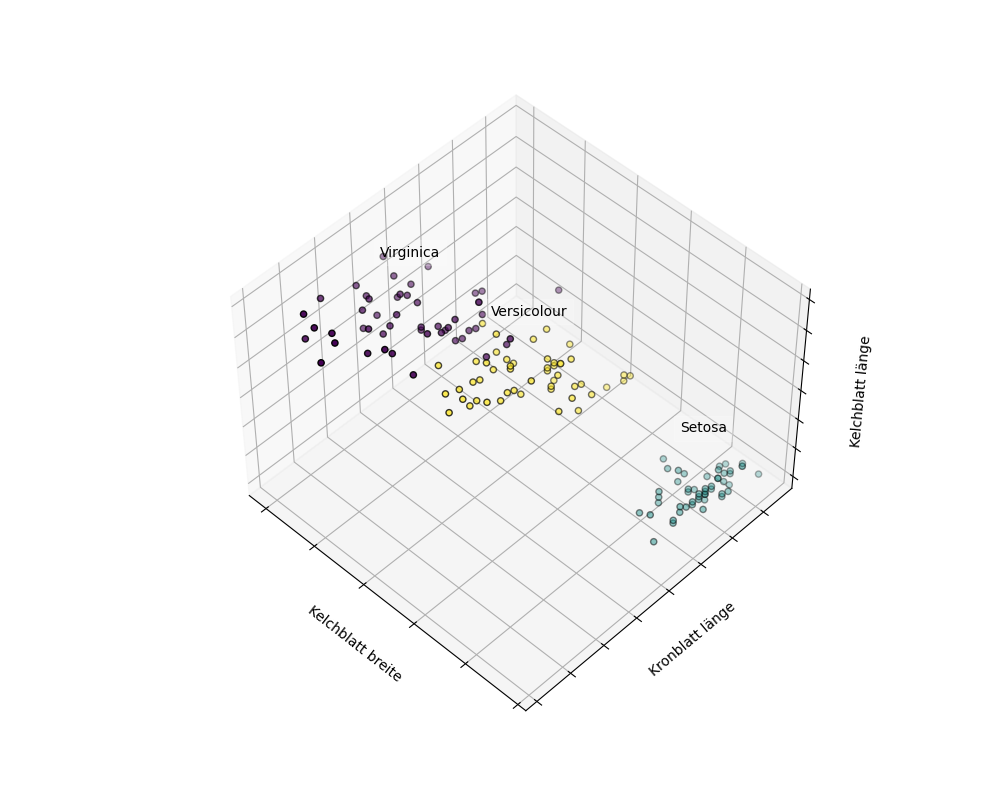
\includegraphics[width=0.9\textwidth]{graphics/iris_set_groundtruth.png}
    \centering
    \caption{Die drei beschriebenen Blumengarten aus dem Beispiel Datensatz visualisiert in ihrem jeweiligen Cluster.}
    \label{abb:flower_example}
\end{figure}
Unüberwachte Algorithmen besitzen auch die Fähigkeit, Assoziationen in Datensätzen zu entdecken. Hierbei können die Algorithmen innerhalb eines gewählten Datensatzes zum Beispiel noch unbekannte Zusammenhänge oder Abbildungen zwischen den einzelnen Datenpunkten erkennen und herausfiltern. Solche Zusammenhänge sind dann Eigenschaften wie Muster, welche alle n Datenpunkte auftauchen, oder wie zwischen mehreren Datenpunkten zusammen eine Verbindung steht und dieser Einfluss auf andere Datenpunkte haben. Ein klassisches Beispiel hierfür sind Anzeigen beim Onlinekauf, in welchem Produkte gezeigt werden, welche oft zusammen mit dem gekauft wird, was der Kunde gerade betrachtet.\\
Das letzte Beispiel, die Reduktion der Dimensionen, wird oftmals für die anderen ML Konzepte verwendet. Vor allem bei Algorithmen, welche auf überwachten Lernen basieren kann, ist eine Reduktion der Dimensionen hilfreich, da hierbei die Anzahl der Features reduziert werden kann. Eine reduzierte Anzahl an Features hat damit den Vorteil, dass die Modelle schneller und gegebenenfalls mit höherer Präzision trainiert werden können, da irrelevante Daten durch die Reduktion entfernt werden. Klassisch wird für eine solche Reduktion der Principal Component Analysis (PCA) Algorithmus verwendet. \cite[]{murphy2012machine} \cite[]{FrocMasc2021}

Da die zuvor erwähnten neuronalen Netzwerke für die Implementierung des Agenten verwendet wurden, sollen diese noch einmal zusammengefasst erklärt werden. Reguläre neuronale Netzwerke, in der Literatur auch bekannt als ANNs, bestehen im Grunde immer aus einem Eingang, einer oder mehrerer Schichten und einem abschließenden Ausgang. Komplexerer Varianten von neuronalen Netzwerken existieren in der Form von zum Beispiel rekurrenten neuronalen Netzwerken, welche die Möglichkeit bieten ganze Zeitreihen zu verstehen. Es ist zudem auch möglich mehrerer Eingänge beziehungsweise Ausgänge zu haben, jedoch soll auf diese hier nicht weiter eingegangen werden. Der Eingang eines neuronalen Netzwerkes, oder auch der Input Layer, ist die Stelle an welchem die Daten hineingehen, damit sie dann durch die erste Kante in ein Neuron laufen können. Die Kanten zwischen den einzelnen Neuronen besitzen das komplette antrainierte Wissen, sie können dabei positiv, negativ oder neutral gewichtet sein. Ist eine Kante positiv gewichtet, so hat sie einen erregenden Einfluss auf ein anknüpfendes Neuron. Eine negative Kante hingegen besitzt ein hemmendes Verhalten zum angebundenen Neuron. In einem neutralen Zustand besitzt die Kante keinen Einfluss auf das anschließende Neuron. Innerhalb des Neurons wird nun als Erstes eine Propagierungsfunktion auf die Daten angewendet, welche in den meisten Situationen eine Multiplikation des eigentlichen Wertes mit der Gewichtung der Kante ist. Anschließend folgt eine Aktivierungsfunktion, welche einer differenzierbaren Funktion entspricht. Klassische Aktivierungsfunktionen sind ReLU, Sigmoid oder Tanh. Das Ziel der Aktivierungsfunktionen ist es, dem neuronalen Netzwerk die Möglichkeit zu geben, auch nicht lineare Funktionen abbilden zu können. \cite[]{KrusComp2015}
\begin{figure}[H]
    \includegraphics[scale=1]{graphics/neural_network.pdf}
    \centering
    \caption{Ein einfaches neuronales Netzwerk mit einem Hidden Layer, einem Eingang und einem Ausgang. Der Hidden Layer verwendet eine ReLU Aktivierungsfunktion und die Kanten besitzen unterschiedliche Gewichtung, hier visualisiert durch die Dicke der Kante.}
    \label{abb:nn}
\end{figure}

Für das Training von neuronalen Netzwerken werden sogenannte Optimierer wie Adam, Nadam oder SGD verwendet, welche das Ziel haben, die Kanten und andere Parameter wie einen Bias anzupassen. Die Optimierer unterscheiden sich zueinander unter anderem dadurch, was für eine Implementierung eines Gradientenverfahrens sie verwenden. Dennoch sind die Gradientenverfahren der Kern eines jeden Optimierers und werden verwendet, um den Trainingsprozess eines neuronalen Netzwerkes durchzuführen. Es wurde bereits beschrieben, wie im Grunde beim Training dem Eingang die Features gezeigt werden und gleichzeitig das dazugehörige Label dem Ausgang gezeigt wird. Was jedoch intern passiert, ist, dass eine sogenannte Cost-Function durch die Optimierer untersucht wird. Das Ziel der Optimierer ist es dabei, das lokale oder globale Minimum dieser Funktion zu finden, welche als variablen alle Gewichtungen der Kanten und sonstige Parameter hat. Die Cost-Function beschreibt, wie gut ein neuronales Netzwerk seine Vorhersage für einen beliebigen Datensatz durchgeführt hat und gibt einen numerischen Wert dafür zurück. Mithilfe dieser Bewertung entscheiden die Optimierer dann, inwiefern die einzelnen Gewichtungen angepasst werden müssen, um näher zum Minimum der Cost-Function zu rücken. \cite[]{KrusComp2015}

\newpage
\section{Grundkonzept und Terminologie zum Reinforcement Learning} \label{sec:grundkonzept_rf}
Im Wesentlichen gibt es zwei Elemente, welche zusammen die Grundbasis für alle Arten und Implementierungen im Bereich des Reinforcement Learnings definieren, nämlich der Agent und das Environment. Das Environment bietet dem Agenten eine Umgebung, mit der er interagieren kann. Ein Environment besitzt immer einen State $s$, welcher die kompletten aktuellen Informationen zu einem trägt. Diese Informationen können zum Beispiel im Falle dieser Arbeit die aktuellen Eigenschaften des Schiffs sein, wie die Position, Geschwindigkeit und Beschleunigung. Der Agent besitzt die Möglichkeit in das Environment zu betrachten durch eine Observation $o$, um Informationen aus dem aktuellen State $s$ zu erhalten und damit arbeiten zu können. Die Observation $o$, kann dabei gleich $s$ sein, oder lediglich einer Schnittmenge von $s$ entsprechen. Definiert wird $o$ durch einen Observationspace, welcher festlegt, welche Informationen der Agent aus $s$ entnehmen kann. Im Falle $o=s$, wird von einer vollkommenen Observation gesprochen, wobei $o \cap s$ einer partiellen Observation entspricht. \cite[]{SpinningUp2018} \cite[]{Sutton1998}

\begin{figure}[H]
    \includegraphics[width=\textwidth]{graphics/agent_env_loop.pdf}
    \centering
    \caption{Visualisierung des Agent-Environment Zyklus. Der Agent führt eine Action aus, welche für eine Interaktion mit dem Environment sorgt. Der State des Environments ändert sich und es kann eine Observation mit einem Reward zurück zum Agenten gegeben werden.}
    \label{abb:agent_env_loop}
\end{figure}

Environments bieten dem Agenten eine Anzahl an Aktionen oder Actions $a$ an, welche dem Agenten die Möglichkeit bieten, mit dem Environment zu interagieren und dieses gegebenenfalls durch diese Interaktionen zu verändern. Definiert werden die Actions, welche der Agent treffen kann in dem Actionsspace, welcher sich durch zwei wesentlichen Punkten unterscheiden kann. Der Actionsspace kann definiert werden durch kontinuierlichen oder diskreten Actions. Ein einfaches Beispiel für eine kontinuierliche Action wäre zum Beispiel im Rahmen dieser Arbeit, mit wie viel Grad die momentane Auslenkung des Schiffsruders verändert werden soll. Es wird hierfür ein Bereich definiert zwischen -1 und 1, wobei der Agent dann die Möglichkeit hat, in diesem Bereich frei einen realen Wert zu wählen wie $0.4$ oder $-0.32$. In einem diskreten Actionsspace würde eine Action einem festen ganzen Wert entsprechen. Erneut am Beispiel des Schiffes, könnte diese Action bedeuten, dass das Ruder entweder komplett nach links, oder komplett nach rechts gesetzt wird.

\subsection{Policies}
Welche Action nun der Agent ausführt, hängt davon ab, wie der Agent implementiert wird, und was für Agent es überhaupt ist. Definiert beziehungsweise bestimmt wird die auszuführende Action $a_t$ jedoch bei allen Agenten durch eine Policy, welche deterministisch die Action wählen, markiert durch ein $\mu$,
\begin{align}
    a_t = \mu_\theta(s_t)
\end{align}
oder einen stochastischen Ansatz verfolgen, markiert durch ein $\pi$,
\begin{align}
    a_t \backsim \pi_\theta (\cdot | s_t).
\end{align}
Da eine Policy nicht fest definiert ist, und sich durch verschiedene Parameter unterscheidet, wird zusätzlich ein $\theta$ verwendet, um diese Eigenschaft zu verdeutlichen. Die Parameter $\theta$, welche hierbei gemeint sind, sind zum unter anderem zum Beispiel die Gewichtungen und Bias eines neuronalen Netzwerkes, welches verwendet wird, um die Policy zu beschreiben.

Deterministische Policies sind im Grunde lediglich Abbildungen und es ist klar definiert, welche Action $a$ abhängig vom State $s$ getroffen wird. Stochastische Policices hingegen definieren sich als ein komplexeres Problem und bei ihnen kann in zwei Kategorien unterschieden werden, welche zurückzuführen sind auf den bereits erwähnten, kontinuierlichen oder diskreten Actionspaces. Wird eine Stochastische Policy definiert, so wird im Falle von einem kontinuierlichen Actionsspace, von einer Diagonal Gaussian Policy gesprochen. Hingegen wird von einer Categorial Policy gesprochen, wenn diese in einem diskreten Actionspace definiert wird.

Eine Categorical Policy ähnelt der Struktur eines Classifiers aus dem Bereich der Klassifizierung, wie sie zuvor schon bei der Einführung zum Machine Learning erwähnt wurde. Sie besteht aus einem neuronalen Netzwerk mit einer Architektur aus mehreren Convolutional oder Dense Layern basierend auf dem Datentyp am Eingang, gefolgt von einem Ausgang Layer mit einer Softmax Aktivierungsfunktion Wahrscheinlichkeiten zu erhalten. Jede Wahrscheinlichkeit wird anschließend verwendet, um festzustellen, welche Action nun ausgeführt wird durch entweder ein Sampling oder eine Log-Likliehood. Das Sampling kann in den meisten Fällen durchgeführt werden, durch die verschiedenen Funktionen, welche Machine Learning Bibliotheken wie PyTorch \cite[]{pytorch} anbieten und eine auszuführende Action zurückgeben. Die Log-Likelihood ist definiert durch,
\begin{align}
    \log \pi_\theta (a|s) = \log\left[P_\theta(s)\right]_a.
\end{align}
Wobei das $P_\theta$ dem Vektor entspricht mit den Wahrscheinlichkeiten vom zuvor erwähnten neuronalen Netzwerk. Die Anzahl der Actions ist gleich der Anzahl an Wahrscheinlichkeiten, somit kann eine Action gleichzeitig als Index verwendet werden, um die Log-Likelihood $\log \pi_\theta (a|s)$ einer Action $a$ aus dem Vektor $\log\left[P_\theta(s)\right]$ zu erhalten.

Ein kontinuierlicher Actionsspace und somit eine Diagonal Gaussian Policy beschreibt einen sonderfall einer Gaussischen mehrdimensionalen Normalverteilung. Für einen Actionsspace mit $k$ Dimensionen, einem Mittelwert $\mu = \mu_{\theta}(s)$ und einer Standardabweichung $\sigma = \sigma_{\theta}(s)$ ist die Log-Likelihood beschrieben durch,
\begin{align}
    \log \pi_\theta (a|s) = -\frac{1}{2} \left(\sum_{i = 1}^{k} \left( \frac{(a_i-\mu_i)^2}{\sigma_i^2}+2 \log \sigma_i\right) + k \log 2 \pi \right). \label{eq:dg_log_loglikelihood}
\end{align}
\cite[]{SpinningUp2018}

\subsection{Trajectories}
Die Trajectory $\tau$ im Reinforcement Learning beschreibt eine Sequenz an States und Actions, welcher ein Agent innerhalb eines Environments betrachten und ausführen kann. Definiert wird sie durch Gleichung \ref{eq:trajectory},
\begin{align}
    \tau = (s_0, a_0, s_1, a_1, \dots) \label{eq:trajectory}.
\end{align}
Eine weitere Art die Trajectory zu definieren folgt durch,
\begin{align}
    \tau = (s_0, a_0, r_0, s_1, a_1, r_1, \dots) \label{eq:trajectory_r},
\end{align}
wobei $r$ hier dem Reward entspricht, auf welchem im nächsten Unterkapitel \ref{sec:reward} näher eingegangen wird.\\
Der allererste State innerhalb eines Environments wird innerhalb der Trajectory zufällig gewählt, durch eine Start-State Verteilung $\rho_{\theta}$, welche definiert ist durch die folgende Gleichung \ref{eq:ss_distribution},
\begin{align}
    s_0 \backsim \rho(\cdot) \label{eq:ss_distribution}.
\end{align}
Was nun genau passiert, wenn der Agent eine Action ausführt und somit der State $s_t$ des Environments übergeht zum State $s_{t+1}$ wird beschrieben durch die sogenannte State Transition, welche wie auch schon die Policies deterministisch oder stochastisch abfolgen kann. Ob sie jetzt deterministisch oder stochastisch ist, hängt vom Environment selbst ab und wie dieses definiert ist. Die State Transition für den deterministischen Fall beschreibt sich durch Gleichung \ref{eq:st_dete},\begin{align}
    s_{t+1} = f(s_t, a_t) \label{eq:st_dete}
\end{align}
wobei hingegen der Stochastische Fall sich beschreibt durch die folgende Gleichung,
\begin{align}
    s_{t+1} \backsim P(\cdot | s_t, a_t) \label{eq:st_stoch}.
\end{align}

\subsection{Reward und Return Functions} \label{sec:reward}
Der Reward $r$ spielt eine sehr entscheidende Rolle und ist eines der wichtigsten Konzepte im Reinforcement Learning. Für den Agenten ist dieser Reward insofern wichtig, da dieser die treibende Kraft für ihn ist. Abhängig davon, was für eine Trajectory der Agent wählt, hat er das Ziel den Reward, beziehungsweise die kumulative Summer aller Rewards einer Trajectory zu maximieren. Definiert wird der Reward durch Gleichung \ref{eq:reward_function},
\begin{align}
    r_t = R(s_t, a_t, s_{t+1}) \label{eq:reward_function}.
\end{align}
Wobei hier anzumerken ist, dass in diesem Fall eine Definition verwendet wurde, welche sowohl den State $s_t$, die dazugehörige Action $a_t$ und den nächsten State $s_{t+1}$ verwendet. Es gibt Alternativen hierfür, wie sie auch unter anderem im Modell dieser Arbeit verwendet wurden. Diese Alternativen unterscheiden sich dabei dadurch, dass zum Beispiel lediglich eine Abhängigkeit zum State $s_t$ steht, $r_t = R(s_t)$, oder eben nur das State-Action Paar verwendet wird $r_t = R(s_t, a_t)$. In dieser Arbeit wurde die Definition verwendet, welche sowohl den State $s_t$ beziehungsweise eine Observation zusammen mit einer Action $a_t$ einschließt. Mehr dazu folgt allerdings in späteren Kapitel. Wie zuvor erwähnt, hat der Agent das Ziel, die kumulative Summe aller Rewards abhängig von einer Trajectory zu maximieren. Die Methode, wie nun diese kumulative Summe bestimmt wird, ist davon abhängig, wie weit in die Zukunft geschaut werden soll vom Agenten. Hierfür wird unterschieden zwischen sogenannten Finite-Horizon Discounted Returns oder Infinite-Horizon Discouted Returns. Beide sind definiert durch die folgenden Gleichungen,
\begin{align}
    R(\tau) = \sum_{t = 0}^{T} r_t \label{eq:finite_horizon_undiscounted}
\end{align}
und
\begin{align}
    R(\tau) = \sum_{t = 0}^{\infty} \gamma^t r_t. \label{eq:infinite_horizon_discounted}
\end{align}
Werden beide Gleichungen betrachtet und verglichen, so fällt auf, dass ein $\gamma^t$ in Gleichung \ref{eq:infinite_horizon_discounted} verwendet wird und die Summe in die Unendlichkeit läuft. Hingegen existiert dieses $\gamma$ für Gleichung \ref{eq:finite_horizon_undiscounted} nicht und die Summe läuft stattdessen lediglich gegen einen Wert $T$. Das $\gamma$ entspricht dem Discount Factor, welcher manuell als Hyperparameter gesetzt werden kann und somit die Möglichkeit bietet zu wählen, wie relevant spätere Rewards innerhalb einer Trajectory sind. Die zwei Discount Functionen bieten den Vorteil, dass sie einerseits die Implementierung vereinfachen, da nun nicht mehr unendlich lange Summen gebildet werden müssen, welche unter Umständen nicht Konvergieren. Nicht konvergierende Endwerte sorgen für eine Anzahl an Problemen beim Implementieren und dieses Problem wird somit elegant umgangen. Elegant vor allem durch den zweiten Vorteil, welcher zuvor schon einmal kurz erwähnt wurde, nämlich dass spätere Rewards für den Agenten an Relevanz verlieren, da diese kaum noch Wirkung auf die Gesamtsumme haben. Ein Resultat hierdurch ist, dass der Agent vermehrt einen Greedy-Algorithmus entspricht und es somit bevorzugt schnell großen Reward zu bekommen. \cite[]{SpinningUp2018} \cite[]{Sutton1998}

\subsection{Reinforcement Learning im Gesamten}
Die Ideen der Policies, Trajectories und auch der Reward Functionen können nun zusammengesetzt werden, um Reinforcement Learning als gesamtes zu definieren. Reinforcement Learning definiert oder beschreibt ein Optimierungsproblem, welches das Ziel hat, die richtige Policy zu wählen, um den gesamten erwarteten Return aus den Rewards einer Trajectory zu maximieren.

Wird ein Environment betrachtet, in welchem sowohl die Policy als auch die Transisitons stochastisch sind, so definiert sich Wahrscheinlichkeit für eine Trajectory mit $T$ Schritten durch Gleichung die folgende Gleichung \ref{eq:prob_of_step_trajectory},
\begin{align}
    P(\tau | \pi) = \rho_0(s_0) \prod _{t = 0}^{T-1} P\left(s_{t+1}|s_t,a_t\right)\pi(a_t|s_t). \label{eq:prob_of_step_trajectory}
\end{align}
Weiterführend wird unter Verwendung von Gleichung \ref{eq:prob_of_step_trajectory} nun der erwartete Return $J(\pi)$ definiert durch
\begin{align}
    J(\pi) = \int_{\tau}^{} P(\tau | \pi) R(\tau) = \underset{\tau \backsim \pi}{E}\left[R(\tau)\right]. \label{eq:expected_return}
\end{align}
Das Optimierungsproblem kann somit zusammengefasst werden durch,
\begin{align}
    \pi^* = \arg \underset{\pi}{\max} J(\pi) \label{eq:optimized_problem}
\end{align}
wobei $\pi^*$ der optimalen Policy, also der Policy entspricht mit dem größten erwarteten Reward. \cite[]{SpinningUp2018} \cite[]{Sutton1998}

\subsection{Value Functions}
Viele Reinforcement Learning Algorithmen verwenden sogenannte Value Functions, welche die Aufgabe haben dem Agenten einen Weg zu bieten, einen State in dem er sich gerade befindet zu bewerten. Außerdem gibt sie dem Agenten die Möglichkeit zu bewerten, wie gut eine die potenzielle Ausführung einer Action im momentanen State ist. Eine solche Bewertung beträgt als quantitative Größe dabei den erwarteten Reward. Unterschieden werden kann die Value Function in vier verschiedene Typen. Der erste Typ, die sogennante On-Policy Value Function $V^{\pi}(s)$ beschrieben in Gleichung \ref{eq:on_policy_value_function}, gibt den erwarteten Reward zurück für den Fall, dass mit einem State $s$ gestartet wird und immer nach der Policy $\pi$ agiert wird.
\begin{align}
    V^{\pi}(s) = \underset{\tau \backsim \pi}{E}\left[R(\tau)|s_0 = s\right] \label{eq:on_policy_value_function}
\end{align}
Der zweite Typ, in der Literatur beschrieben als die On-Policy Action-Value Function $Q^{\pi}(s,a)$, sieht dem ersten Typ ziemlich ähnlich und der Name deutet schon an, wo genau der Unterschied liegt. Typ zwei, beschrieben durch Gleichung \ref{eq:on_policy_action_value_function}, verwendet außerdem eine Action $a$ zusammen mit State $s$, um eine Bewertung für den aktuellen State $s$ zu ermitteln. Der erwartete Reward wird hier dadurch gebildet, dass die potenziell unabhängig von der Policy $\pi$ Action $a$ ausgeführt wird zum Start mit State $s$, nach dem Start wird dann regulär nach der Policy $\pi$ agiert und fortgefahren.
\begin{align}
    Q^{\pi}(s,a) = \underset{\tau \backsim \pi}{E}\left[R(\tau)|s_0 = s, a_0 = a\right] \label{eq:on_policy_action_value_function}
\end{align}
Für den Fall, dass die optimale Policy verwendet wird und lediglich in State $s$ gestartet wird, ohne eine Action $a$ in Betracht zu ziehen, wird folgende Gleichung $V^*(s)$ definiert,
\begin{align}
    V^{*}(s) = \underset{\pi}{\max}\underset{\tau \backsim \pi}{E}\left[R(\tau)|s_0 = s\right]. \label{eq:optimal_value_function}
\end{align}
Analog zum vorherigen Fall existiert auch hier wieder eine Variante wie in Gleichung \ref{eq:on_policy_action_value_function}, welche in State $s$ startet und außerdem eine gegebenenfalls zu $\pi^*$ unabhängige Action $a$ ausführt und anschließend der optimalen Policy $\pi^*$ folgt. Definiert ist diese durch die folgende Gleichung \ref{eq:optimal_action_value_function},
\begin{align}
    Q^{*}(s,a) = \underset{\pi}{\max}\underset{\tau \backsim \pi}{E}\left[R(\tau)|s_0 = s, a_0=0\right]. \label{eq:optimal_action_value_function}
\end{align}
Zwischen der optimalen Q-Function $Q^*(s,a)$ und der von der optimalen Policy $\pi$ gewählten Action $a$ existiert ein Zusammenhang, welcher beschrieben wird durch Gleichung \ref{eq:optimal_action_q_function}.
\begin{align}
    a^*(s) = \arg \max_a Q^* (s,a) \label{eq:optimal_action_q_function}
\end{align}
Per Definition wählt die optimale Policy $\pi^*$ stets die Action in einem momentanen State, welche den besten erwarteten Reward liefert. Der erwartete Reward ausgehend von der optimalen Q-Funktion $Q^*(s,a)$, wird bestimmt auf Basis eines start States $s$ und einer Action $a$ und dem anschließenden Ausführen von Actions ausgehend der optimalen Policy. Es ist somit möglich, die optimale Action $a^*$ zu bestimmen durch Gleichung \ref{eq:optimal_action_q_function}, ohne dass der Agent ein Wissen darüber haben muss, was für States und deren Wert in zukunft folgen. \cite[]{SpinningUp2018} \cite[]{Sutton1998}

\subsection{Bellman Gleichungen}
Der Agent oder die Policy soll die Fähigkeit besitzen seinen aktuellen State $s$ zu bewerten, um damit aussagen zu können, ob er sich momentan in einem guten State befindet, oder nicht. Geschehen kann dies durch die zuvor definierten Value Functions, welche einen State verwenden können, mit gegebenenfalls einer Action, um einen erwarteten Reward zu bestimmen. Möchte der Agent nun wissen, wie der nächste State aussehen würde, so fällt ihm dies sehr schwer, da er seine verschiedenen Actions nutzen müsste, um eine Transition in den nächsten State auszulösen. Abhilfe für dieses Problem sollen die Bellman Gleichungen bieten, welche eine formale Verbindung zwischen der Bewertung des aktuellen States und der Bewertung der nächsten States herstellen sollen. Grundsätzlich sagen sie aus, dass der Wert des aktuellen Startpunktes gleich dem erwarteten Reward plus dem Wert des States ist, auf welchem er als Nächstes kommt. Für die On-Policy Value Functions sind die Bellman Gleichungen $V^{\pi}(s)$ und $Q^{\pi}(s)$ definiert durch die beiden Gleichungen \ref{eq:bellman_v_on_policy} und \ref{eq:bellman_q_on_policy}.
\begin{align}
    V^{\pi}(s) = \underset{\underset{s' \backsim P}{a \backsim \pi}}{E}\left[r(s,a)+\gamma V^{\pi}(s')\right] \label{eq:bellman_v_on_policy}
\end{align}

\begin{align}
    Q^{\pi}(s,a) = \underset{s' \backsim P}{E}\left[r(s,a)+\gamma \underset{a' \backsim \pi}{E}\left[Q^{\pi}(s',a')\right] \right] \label{eq:bellman_q_on_policy}
\end{align}
Das in den Gleichungen vorkommende $s'$ beschreibt den nächsten State folgend auf State $s$, welches durch Transition $s' \backsim P = s' \backsim P(\cdot |s,a)$ gewählt wird. Die Bellman Gleichungen für die optimalen Wert Funktionen oder Value Functions werden durch die folgenden zwei Gleichungen beschrieben,
\begin{align}
    V^*(s) = \max_a \underset{s'\backsim P}{E}\left[r(s,a)+\gamma V^s(s')\right] \label{eq:bellman_opv_on_policy}
\end{align}
und
\begin{align}
    Q^*(s,a) = \underset{s' \backsim P}{E}\left[r(s,a)+\gamma \max_{a'}Q^*(s', a')\right]. \label{eq:bellman_opq_on_policy}
\end{align} \cite[]{SpinningUp2018}

\section{Arten des Reinforcement Learnings TODO} \label{sec:arten_rf}
Im Reinforcement Learning gibt es eine ganze Reihe an verschiedenen Arten und Implementationen von Algorithmen. Im groben kann jedoch schon dadurch entschieden werden, ob es sich um Model-Free oder Model-Based Reinforcement Learning handelt. Eine allgemeine Übersicht soll Abbildung \ref{abb:rl_overview} bieten. Hier sind die Model-Free Algorithmen auf der linken Seite zu erkennen, während die Model-Based Algortihmen auf der rechten Seite liegen.
\begin{figure}[H]
    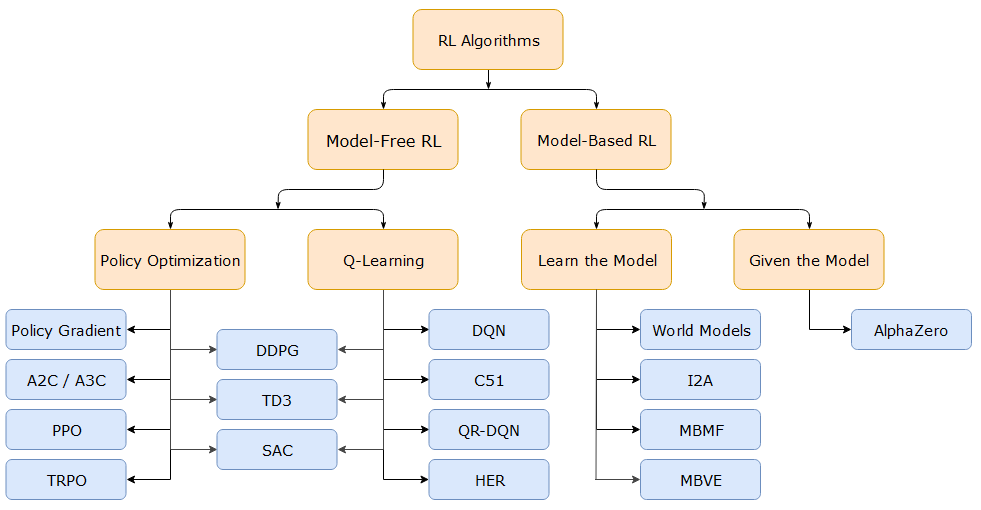
\includegraphics[width=\textwidth]{graphics/rl_overview.png}
    \centering
    \caption{Übersicht der verschiedenen Reinforcement Learning Algorithmen und wo sie sich einordnen. \cite[]{SpinningUp2018}}
    \label{abb:rl_overview}
\end{figure}
Wird ein Agent in einem Modell oder Environment implementiert wie es in dieser Arbeit zum Beispiel der Fall mit dem Schiffsmodell ist, so sagt dieses nicht aus, dass nun ein Model-Based Algorithmus verwendet wird. Es sagt auch nicht direkt aus, ob nun ein Model-Free Algortihmus verwendet wurde. Beide Begriffe deuten auf die Art des Lernens und eine gewisse Eigenschaft, welche jedes Environment, oder zum Beispiel Kräftemodell aus der Regelungstechnik anbieten kann. Beide Begriffe sollen somit nicht verwechselt werden mit den Modellen aus der Regelungstechnik, beziehungsweise dem Environments, in welchen der Agent agiert.

Grundsätzlich sagen die Begriffe Model-Free und Model-Based aus, wie ein jeweiliger Algorithmus seine Entscheidung trifft. Ein Algorithmus welcher auf einem Model-Based Ansatz implementiert ist, besitzt die Möglichkeit mehr oder weniger ein Modell beziehungsweise eine Funktion zu befragen, was passieren würde, wenn nun Action $a$ ausgeführt wird. Die Antwort auf eine solche Frage, kann dann Informationen sein, wie der potenzielle Reward, wenn Action $a$ auch wirklich ausgeführt wird. Model-Based Algorithmen verfügen somit also über die besondere Funktion, vorraus zu planen und genau zu wissen was passiert, wenn verschiedene Actions ausgeführt werden. Ausgewählt werden kann dann die Action, welche letztendlich den besten gesamt Reward liefert.

\section{Soft Actor-Critic (SAC) Agenten} \label{sec:howto_sac}
Der Soft Actor-Critic (SAC) Algorithmus ist jener, welcher für das Regeln beziehungsweise Kontrollieren des dynamischen Modells in dieser Arbeit verwendet wurde. Er findet sich in der Gruppe der Model-Free RL Algorithmen wieder und basiert zum Teil auf Ideen aus früheren Algorithmen wie DDPG und soll eine Kombination aus den Vorteilen dieser darstellen.

Model-Free RL Algorithmen haben immer mit zwei großen Herausforderungen gekämpft, welche ihre Performanz deutlich reduziert haben. Die erste der beiden Herausforderungen ist die Sample Komplexität. So hatten sogar kleine Aufgaben das Problem, dass sie bereits Millionen von Datenpunkten brauchen. Die zweiten große Herausforderungen ist die Instabilität, welche bisherige Algorithmen mit sich gebracht haben. So konnten Probleme durchaus mit RL Algorithmen gelöst werden, änderte sich das Problem jedoch minimal, so versagten die RL Algorithmen bereits. \cite[]{sacv2}

SAC löst diese Herausforderungen, in dem es Konzepte aus anderen Algorithmen verwendet und diese kombiniert, um eine Brücke zwischen Stochastischen Policy Optimierungen und DDPG Algorithmen herzustellen. Außerdem werden die Vorteile aus anderen Algorithmen verwendet, wie der Replay Buffer, um auf vergangene Transitions zugreifen zu können, oder die Verwendung des dualen Critic-Netzwerk Tricks. \cite[]{brockman2016openai}

Das zentrale neue Konzept, welcher den SAC definiert und auch für die Namensgebung sorgt, ist die Idee der Entropy Regularization. Während reguläre RL Algorithmen oft lediglich das Ziel haben, zu versuchen den Reward beziehungsweise den erwarteten Reward zu maximieren, hat der SAC außerdem einen Entropy Anteil neben dem Reward. Das Ziel des SAC ist es somit, sowohl den Reward als auch die Entropy zu maximieren. So wird die Entropy $\mathcal{H}(\pi(\cdot | s_t))$ hier definiert durch,
\begin{align}
    \mathcal{H}(\pi(\cdot | s_t)) = \mathbb{E}_{a\backsim \pi(\cdot | s)}[-\log(\pi(a|s))],
\end{align}
und erweitert die Optimale Stochastische Policy dementsprechend im Reward Anteil,
\begin{align}
    \pi^* = \arg \max_{\pi} \underset{\tau \backsim \pi}{E} \left[\sum_{t=0}^{\infty} \gamma^t\left(R(s_t, a_t, s_{t+1}) + \alpha \mathcal{H}(\pi(\cdot | s_t))\right)  \right].
\end{align}
Der Temperatur Parameter $\alpha > 0$, kontrolliert die relative Gewichtung der Entropy $\mathcal{H}$ im Vergleich zum herkömmlichen Reward $r$ und wird somit als einer der Hyperparameter betrachtet, welcher beim Trainieren der Modelle angepasst und optimiert werden muss. Eine Optimierung der Größe ist daher wichtig, da jedes Environment sich voneinander unterscheidet. Der Temperatur Parameter dient gleichzeitig auch als der Parameter, welcher kontrolliert, ob der SAC versucht das bisherige Wissen mehr auszunutzen, oder ob er versucht neue Wege versucht zu finden, um seinen erwarteten Reward zu erhöhen. So bedeutet ein hoher Wert für $\alpha$, dass der SAC mehr Erkundung nach neuen Wegen durchführt, hingegen sorgt ein niedriger Wert dazu, dass der SAC eher auf bereits bekanntes Wissen setzt.

Durch die Einführung der Entropy in die Policy, verändert sich auch die Value Function und wird erweitert durch dem Entropy Term,
\begin{align}
    V^{\pi}(s) = \underset{\tau \backsim \pi}{E}\left[\sum_{t = 0}^{\infty} \gamma^t\left(R(s_t, a_t, s_{t+1}) + \alpha \mathcal{H}(\pi(\cdot | s_t))\right) \vert  s_0 = s \right].
\end{align}
Abschließend wird auch die Q-Function erweitert um den Entropy Term zusammen mit seinem Temperatur Parameter,
\begin{align}
    Q^{\pi}(s, a) = \underset{\tau \backsim \pi}{E}\left[\sum_{t = 0}^{\infty} \gamma^t R(s_t, a_t, s_{t+1}) + \alpha \sum_{t = 1}^{\infty} \gamma^t \mathcal{H}(\pi(\cdot | s_t)) \vert s_0 = s, a_0 = a \right].
\end{align}
Die neuen Definitionen für die Value Function und Q-Function können nun vereint werden und letztendlich verwendet werden, um die Bellman Gleichung \ref{eq:bellmansac} für den SAC aufzustellen. \cite[]{sacv2} \cite[]{brockman2016openai}
\begin{align}
    V^{\pi}(s) = \underset{a \backsim \pi}{E} \left[Q^{\pi}(s, a)\right] + \alpha \mathcal{H}(\pi(\cdot | s)) \label{eq:value_sac}
\end{align}

\begin{align}
    Q^{\pi}(s,a) & = \underset{a' \backsim \pi}{\underset{s' \backsim P}{E}} \left[R(s, a, s') + \gamma (Q^{\pi}(s', a') + \alpha \mathcal{H}(\pi(\cdot | s')))\right] \\
                 & = \underset{s' \backsim P}{E} \left[R(s,a,s') + \gamma V^{\pi}(s')\right]. \label{eq:bellmansac}
\end{align}

Beim Lernprozess des SAC, werden sowohl die Policy $\pi_{\theta}$, als auch die beiden Critic-Netzwerke beziehungsweise Q-Functions $Q_{\phi_1}$ und $Q_{\phi_2}$ optimiert. Je nachdem, welche Version vom SAC verwendet wird, unterscheidet sich der Lernprozess ein wenig. Fokussiert werden soll hier jedoch auf die 2. Version, welche bereits den dualen Critic-Netzwerk Trick verwendet und außerdem noch das Value Function Netzwerk besitzt, um einen State zu bewerten. Die neuste Version des SAC besitzt dieses Value Function Netzwerk nicht mehr, da Erfahrungen gezeigt haben, dass dieses nicht wirklich relevant für die Erzeugung von Ergebnissen ist. \cite[]{sacv3}

Der Lernprozess selbst ist hierbei ziemlich ähnlich zu dem des TD3 Algorithmus, welcher im Grunde einem SAC Algorithmus entspricht, wenn alle Stochastischen Eigenschaften entfernt werden. Die beiden Q-Functions werden optimiert, beziehungsweise lernen durch die Mean-Squared Bellman Error (MSBE) Minimierung des Losses $L(\phi_i, \mathcal{D})$ mit einem Targetnetzwerk $y(r, s', d)$,
\begin{align}
    L(\phi_i, \mathcal{D}) = \underset{(s, a, r, s', d) \backsim \mathcal{D}}{E}\left[\left(Q_{\phi_i}(s,a) - y(r, s', d)\right)^2 \right]
\end{align}
wobei das Targetnetzwerk gegeben ist durch,
\begin{align}
    y(r,s', d) = r+\gamma(1-d)\left(\min_{j=1,2}Q_{targ,j}(s', \widetilde{a}')-\alpha \log \phi_{\theta}(\widetilde{a}' | s')\right), \widetilde{a}'\backsim \pi_{\theta}(\cdot |s').
\end{align} \label{eq:target}
Es wird am Ende die Q-Function vom SAC Algorithmus verwendet, welche den kleineren Loss $L(\phi_i, \mathcal{D})$ besitzt.

Die Policy $\pi_{\theta}$ des SAC hat das Ziel, für jeden State den erwarteten Reward und die erwartete Entropy zu maximieren, somit hat sie das Ziel die Value Function $V^{\pi}(s)$ zu maximieren, wie sie bereits zuvor in Gleichung \ref{eq:value_sac} definiert wurde. Diese wird nun umgeschrieben zu,
\begin{align}
    V^{\pi}(s) = \underset{a \backsim \pi}{E} \left[Q^{\pi}(s, a)\right] - \alpha \log(\pi(a | s)) \label{eq:value_sac2}
\end{align}
diese Umwandlung der Value Function $V^{\pi}(s)$ hat den Zweck, das nun ein sogenannter Reparameterisation Trick angewendet werden kann. Das Ziel des Tricks ist es die Möglichkeit zu besitzen, nun nicht mehr Abhängig von den Parametern $\theta$ zu sein. Durch diesen Trick werden die Action $a$ nun gesampled durch eine Squashed Guassian Policy,
\begin{align}
    \widetilde{a}_\theta(s, \zeta) = \tanh(\mu_\theta(s) + \sigma_\theta(s) \odot \zeta), \zeta \backsim \mathcal{N} (0, I) \label{eq:reparamtrick}
\end{align}
was zur Folge hat, das auch in $V^{\pi}(s)$ unabhängig von $\theta$ die Action $\widetilde{a}_\theta(s, \zeta)$ gesampled wird,
\begin{align}
    V^{\pi}(s) = \underset{\zeta \backsim \mathcal{N} }{E} \left[Q^{\pi\theta}(s, \widetilde{a}_\theta(s, \zeta)) - \alpha \log\pi_\theta(\widetilde{a}_\theta(s, \zeta) | s)\right]
\end{align}
Abschließend, damit nun auch der tatsächliche Policy Loss bestimmt werden kann, muss nur noch das $Q^{\pi\theta}$ substituiert werden durch einen Approximierer,
\begin{align}
    \max_\theta \underset{\underset{\zeta \backsim \mathcal{N} }{s \backsim \mathcal{D} }}{E} \left[\min_{j=1,2}Q_{\phi_j}(s,\widetilde{a}_\theta(s, \zeta)) - \alpha \log \pi_\theta(\widetilde{a}_\theta(s, \zeta)|s)\right].
\end{align}
\cite[]{sacv2} \cite[]{brockman2016openai}

\newpage
Eine Übersicht über den kompletten Lernprozess des SAC, soll noch einmal in dem folgenden Pseudocode gezeigt werden,
\begin{algorithm}[H]
    \caption{Soft Actor-Critic Algorithmus}\label{pse:sac_pseudo}
    \begin{algorithmic}[1]
        \State Initialisiere Policy $\pi$ Parameters $\theta$, Q-Functions/ANN Parameter $\phi_1, \phi_2$ und den Replay Buffer $\mathcal{D}$
        \State Setze Targetnetzwerk Parameter gleich den Hauptparametern $\phi_{targ,1} \leftarrow \phi_1, \phi_{targ,2} \leftarrow \phi_2$
        \For{Iteration}
        \State Observiere State $s$ und wähle Action $a \backsim \pi_{\theta}(\cdot | s)$
        \State Führe Action $a$ aus und sorge für State Transition zu $s'$
        \State Observiere State $s'$, Reward $r$ und das Episoden Signal $d$
        \State Speicher $(s, a, r, s', d)$ im Replay Buffer $\mathcal{D}$
        \If{$d = \text{True}$}
        \State Beende frühzeitig, da Episode zuende und setze Environment zurück
        \EndIf
        \If{Zeit für Updates}
        \For{$j$ in $n$-Updates}
        \State Nehme ein Batch von Transitions $B = \left\{(s, a, r, s', d)\right\}$ aus $\mathcal{D}$
        \State Bestimmte Targets $y$ für Q-Functions nach Gleichung \ref{eq:target}
        \State Update die Q-Functions durch Gradientenverfahren um einen Schritt
        \State Update die Policy durch Gradientenverfahren um einen Schritt
        \State Update die Targetnetzwerke
        \EndFor
        \EndIf
        \EndFor
    \end{algorithmic}
\end{algorithm}

\chapter{Methode und Umsetzung} \label{sec:methode_umsetzung}

\section{Verwendete Software und Bibliotheken} \label{sec:software_bibs}
Der Großteil der ganzen Arbeit wurde mithilfe der Programmiersprache Python \cite[]{python} umgesetzt. Python bietet den Vorteil an, dass es vergleichsweise eine recht einfache Sprache ist und außerdem eine ziemlich große Auswahl an Bibliotheken im Bereich Machine Learning bietet. Die verwendete Machine Learning Bibliothek in dieser Arbeit ist PyTorch \cite[]{pytorch}. PyTorch ist ein Framework, mit welchem die neuronalen Netzwerke für den Agenten einfach und mit viel Freiheit definiert werden können. So können zum Beispiel die Forward Function, oder die Learn Function des neuronalen Netzwerks frei, und mit kompletter Kontrolle definiert werden. Grafiken und die Videodateien, welche für die Visualisierung und Auswertung einer Episode verwendet werden, wurden mithilfe der Matplotlib \cite[]{matpltlib} Bibliothek generiert. Da der Agent zwingend ein Environment benötigt, in welchem das dynamische Modell simuliert werden kann, wurde zusätzlich die Bibliothek Gym von OpenAI \cite[]{brockman2016openai} verwendet. Gym bietet ein Framework an, welches dem Benutzer mit vordefinierten Functions die Möglichkeit bietet, Environment zu erstellen. So werden zum Beispiel die Step, oder Reset Function vorgegebene, welche dazu verwendet werden, um einen Zeitsprung innerhalb einer Episode durchzuführen. Im Falle der Reset Function würde das Environment wieder auf seinen Ursprungsstate zurückgesetzt werden. Dies bedeutet, dass Eigenschaften des Environments, wie die Schiffsposition oder der momentane Reward, wieder auf den Ursprung des Koordinatensystems gesetzt wird beziehungsweise der Reward wieder 0 ist.
\section{Implementierung des Agenten in Python} \label{sec:imp_agent}
Zuvor wurde schon erwähnt, dass für diese Arbeit PyTorch verwendet wird, um den Agenten zu implementieren. Wie genau diese Implementierung nun umgesetzt wurde, soll mit diesem Unterkapitel verdeutlicht werden.

Die erste Komponente des SAC Agenten, soll hier der Replay Buffer $\mathcal{D}$ sein, dieser wurde Implementiert als eine eigene Klasse, welche als Klassenattribute Listen besitzt um die verschiedenen Datenpunkte aus einer Transition $(s, a, r, s', d)$ zu speichern. Zum speichern einer neuen Transisiton wird die Methode \textit{store\_transition} verwendet. Um nun aus dem Replay Buffer einen Batch zu bekommen, wird die Methode \textit{sample\_buffer} verwendet. Das entnehmen, beziehungsweise Sampling erfolgt hierbei zufällig.

Bevor nun die tatsächliche Klasse beschrieben werden kann, welche den Agenten selbst Implementiert. Soll erst einmal auf die verschiedenen neuronalen Netzwerke eingegangen werden, welche mit Hilfe von PyTorch Implementiert wurden. Wie zuvor in der Theorie zum SAC, werden ingesamt drei Arten von neuronalen Netzwerken verwendet, das Actor/Policy Netzwerk, die beiden Critic/Q-Function Netzwerke und das Value Netzwerk. Die Netzwerke selbst wurden alle jeweils als eine eigene Klasse implementiert, welche eine \textit{forward} Klassenmethode besitzen um eine propagation der Daten durch die Netzwerke zu ermöglichen. Alle drei Netzwerktypen verwenden die gleiche Grundlegende Netzwerktopologie von zwei auf einander geschichteten Dense Layern mit einer breite von 256 Neuronen. Analog zu den selben Netzwerktopologien, wurden auch in allen drei Fällen die selben Aktivierungsfunktionen und Optimierer verwendet. Für die Aktivierungsfunktionen wird ReLU verwendet, während für die Optimierer der Adam Algorithmus \cite[]{kingma2014method} verwendet wird. Gegeben durch die formale Definition der Policy, variiert das Policy Netzwerk ein wenig im Vergleich zu den anderen beiden Typen. Das Value Netzwerk wird verwendet um sowohl eine Standardabweichung als auch einen Mittelwert zu bestimmen, weshalb es hier zwei Ausgangsneuronen gibt. Bei den anderen beiden Netzwerktypen gibt es hingegen lediglich ein Neuron. Ein weiterer Unterschied bei den äußeren Schichten der neuronalen Netzwerke findet sich außerdem bei den Anzahlen der Eingangsneuronen. Nach formaler Definition benötigen die Critic/Q-Function Netzwerke sowohl den State als auch die Action, während das Value und Policy Netzwerk nur den State benötigt. Alle drei Netzwerktopologien finden sich noch einmal in vereinfachter Version Visualisert in den folgenden drei Abbildungen.

\begin{figure}[H]
    \includegraphics[width=0.7\textwidth]{graphics/critic.pdf}
    \centering
    \caption{Die vereinfachte Topologie des Critic Netzwerkes um die Q-Functions abzubilden. Hier mit dem State und den Actions als Eingangswerte und dem Q-Wert als Ausgang.}
    \label{abb:critic_network}
\end{figure}

\begin{figure}[H]
    \includegraphics[width=0.7\textwidth]{graphics/value.pdf}
    \centering
    \caption{Die vereinfachte Topologie des Value Netzwerkes um die Value-Function abzubilden. Mit dem State als Eingangswert und dem Wert des States als Ausgang.}
    \label{abb:value_network}
\end{figure}

\begin{figure}[H]
    \includegraphics[width=0.7\textwidth]{graphics/policy.pdf}
    \centering
    \caption{Die vereinfachte Topologie des Policy Netzwerkes. Mit dem State als Eingangswert und der Standardabweichung und dem Mittelwerk als Ausgang.}
    \label{abb:policy_network}
\end{figure}

Innerhalb der Klasse, welche das Policy Netzwerk Implementiert, wurde zudem eine weitere Klassenmethode hinzugefügt. Nämlich die \textit{sample\_normal} Klassenmethode, welche genau der Funktion entspricht, welche dem Agenten oder der Policy die Fähigkeit bietet eine Action aus einer Gaussischen Verteilung zu wählen. Desweiteren bietet diese Methode die Möglichkeit eine Log-Likelihood zu ermitteln, welche unteranderem verwendet wird um dann das Target-Value Netzwerk zu aktualisieren während des Lernprozesses.

Die Klasse, welche nun den SAC selbst beschreibt ist aufgebaut, indem zu erst einmal alle vorher Implementierten Netzwerktypen und der Replay Buffer initialisiert werden. Dabei kommen nun die folgenden Netzwerke in Frage,
\begin{enumerate}
    \item[-] Poliy Netzwerk
    \item[-] Critic Netzwerk 1
    \item[-] Critic Netzwerk 2
    \item[-] Value Netzwerk
    \item[-] Target-Value Netzwerk
\end{enumerate}
Für das Sampling, oder wählen einer Action wird die Klassenmethode \textit{choose\_action} definiert, welche als Argument eine Observation verwendet. Die Observation wird innerhalb der Klassenmethode dann an die Klassenmethode \textit{sample\_normal} des Policy Netzwerkes weitergeben, welche die Observation für eine Standardabweichung und einem Mittelwerk durch das Netzwerk propagiert. Mit Hilfe der Standardabweichung und des Mittelwertes kann dann anschließend unter Verwendung des Reparameterisation-Tricks wie beschrieben in Gleichung \ref{eq:reparamtrick} eine Verteilung bestimmt werden, außer welcher dann eine Action genommen wird.

Die Klassenmethode, welche das Updaten des Target-Value Netzwerkes vornimmt, ist Implementiert mit der \textit{update\_network\_parameters} Klassenmethode. Diese wird während des Lernprozesses aufgerufen und kopiert lediglich unter Verwendung der PyTorch Standardmethoden die Netzwerkparameter des Target Netzwerkes zum Target-Value Netzwerk.

Die Klassenmethode \textit{learn}, ist mit die wichtigste Klassenmethode, da sie dem SAC die Möglichkeit bietet überhaupt lernen zu können. Sie funktioniert wie bereits in der Theorie beschrieben, indem zu erst ein Batch aus dem Replay Buffer genommen wird. Der Batch wird anschließend an die verschiedenen Netzwerke weitergegeben, damit die Daten dann durch die Netzwerke propagiert werden können. Anschließend folgen die verschiedenen Schritte definiert in den diversen formalen Gleichungen um die Loss Werte zu bestimmen, die Critic Netzwerke zu vergleichen und letztendlich alle Netzwerke mit den neuen gelernten Informationen anzupassen.

Damit der SAC in seinen internen Replay Buffer schreiben kann, wurde die \textit{remember} Klassenmethode definiert, welche lediglich die Replay Buffer Methode \textit{store\_transition} aufruft und die Transition übergibt. Es existieren außerdem einige Hilfsmethoden, welche dafür sorgen, dass Netzwerke zwischen gespeichert werden können um zu einem späteren Zeitpunkt wieder verwendet werden zu können. Auch diese verwenden erneut die Standardmethoden von PyTorch um die Netzwerkparameter in ein Dictonary zu speichern, welches dann in eine Datei geschrieben wird.

\section{Modellbildung des Schiffs mit Simulink} \label{sec:imp_simulink}
Das in dieser Arbeit verwendete dynamische Modell, soll wie bereits in der Zielsetzung erwähnt ein Kräftemodell sein, welches eine Schiffsfahrt modelliert. Die Grundidee des Modells ist es dabei, dass das Schiff im Ursprung eines Koordinatensystems startet und dann das Ziel hat, innerhalb eines vordefinierten Bereichs nach rechts zu einer Ziellinie zu fahren. Hierbei gibt es das zweitrangige Ziel für das Schiff, dass es bei seiner Überfahrt so mittig im vordefinierten Bereich bleiben soll wie möglich. Die folgende Abbildung \ref*{abb:boat_frame_example_2} soll eine Visualisierung für das gewollte Modell bieten.
\begin{figure}[H]
    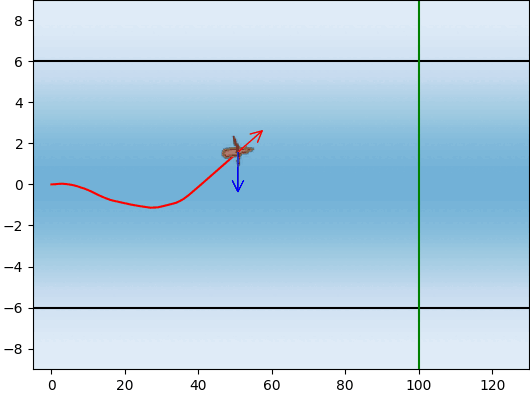
\includegraphics[width=\textwidth]{graphics/boat_frame_example_2.png}
    \centering
    \caption{Visualisierung des Schiff-Agentens während einer Überfahrt mit Windeinfluss (Blauer Pfeil) und Richtungs-Vektor (Roter Pfeil). Zusehen sind außerdem die Windkurven für die Windgeschwindigkeit und dem Winkel von wo der Wind weht. Ein Winkel von $\frac{\pi}{2}$ würde einer Windrichtung von unten innerhalb der Abbildung bedeuten.}
    \label{abb:boat_frame_example_2}
\end{figure}
In Abbildung \ref*{abb:boat_frame_example_2} ist zu erkennen, wie das Schiff eine grüne Ziellinie hat, welche es unbedingt erreichen soll, damit eine Episode innerhalb des Reinforcement Learnings erreicht ist. Außerdem ist durch schwarze Linien ein äußerer Bereich gekennzeichnet, welches das Schiff nicht überschreiten soll. Ein Überschreiten führt beim Training des Agenten zu einer frühzeitigen Beendigung der Episode. Des Weiteren soll eine Störgröße das Schiff beziehungsweise den Agenten bei seiner Überfahrt beeinflussen, damit der Agent lernen soll, diese Störgröße automatisch auszugleichen. Die Störgröße in Form von einem Wind im Modell vorhanden sein, der Wind kann dabei aus jeder Richtung wehen und verändert sich mit der Zeit in der Richtung und in der Windgeschwindigkeit.\\
Die Modellbildung selbst findet nun statt aus der Perspektive des Schiffs, die tatsächliche Kinematik, sprich zum Beispiel die tatsächliche Richtung, in welche sich das Schiff dann im Environment bewegt wird in einem späteren Schritt dann umgerechnet.

Die größte Inspiration für die Modellbildung kommt aus dem Beitrag von Knud Benedict \& Matthias Kirchhoff, welche zusammen eine Einführung in die Modellbildung für Schiffe und deren Dynamik in ihrer Veröffentlichung \glqq Explaining Ships Dynamic and Handling Using MATLAB \& SIMULINK as Simulation Tool in Teaching Maritime Students\grqq{} \cite[]{Benedict2007ExplainingSD} bieten. Das Schiff wird in diesem Modell durch drei Bewegungsgleichungen modelliert, welche die Kräfte in longitudinaler, transversaler und das Giermoment des Schiffs beschreiben. Visualisiert sind diese in Abbildung \ref{abb:ship_eoms}.
\begin{figure}[H]
    \includegraphics[width=0.8\textwidth]{graphics/ship_eoms.pdf}
    \centering
    \caption{Die drei Bewegungsgleichungen, welche das Kräftemodell aus der Perspektive des Schiffs modellieren.}
    \label{abb:ship_eoms}
\end{figure}

\subsection{Verwendete Konstanten und Parameter in der Modellbildung}
Für die Modellbildung wurden verschiedene Konstanten, Koeffizienten und Parameter verwendet, welche sowohl aus Quellen stammen, als auch durch eigenes Experimentieren bestimmt wurden. Experimentell bestimmte Werte wurden frei nach eigenem Gefühl gewählt und rein davon abhängig gemacht, inwiefern das Modell sich innerhalb einer Simulink Simulation verhalten hat. So wurde die Masse des Schiffs zum Beispiel so angepasst, dass es einem \glqq realistischem\grqq{} Verhalten nachahmt, wenn eine Kurve gefahren wird. Wird die Masse jedoch verglichen mit der Propellerlänge, so ist schnell zu erkennen, das diese ziemlich unrealistisch erscheint. Eine perfekte Modellierung eines Schiffes würde jedoch leider über diese Arbeit hinausgehen, und sie erscheint auch nicht als nötig. Das bestehende Modell wirkte sich als mehr als ausreichend für die Experimente, welche durchgeführt wurden, um die Anwendung des Reinforcement Learning Agenten zu testen.

Die verwendeten Konstanten und Koeffizienten finden sich in der folgenden Tabelle \ref{tab:constants} wieder. Werte, die für dieses Modell durch Experimentieren bestimmt wurden, sind markiert durch ein [E]. Jene Werte, die sowohl ein [E] wurden experimentell angepasst, basieren aber aus Inspiration aus der jeweiligen Quelle, um einen Richtwert zu haben.
\begin{table}[H]
    \begin{tabular}{l|l}
        $\rho = \SI{1}{\kg\per\cubic\m}$ & Dichte von Wassers                                                                 \\ \hline
        $d = \SI{1}{\m}$                 & Durchmesser des Propellers [E]                                                     \\ \hline
        $n = \SI{30}{\per\minute}$       & Drehgeschwindigkeit des Propellers [E]                                             \\ \hline
        $t = 0.3$                        & Leistungsabzug der Schraube \cite[]{Zelazny_2014} \cite[]{Kulczyk_Tabaczek_2014_2} \\ \hline
        $w = 0.3$                        & Nachlaufströmungs Koeffizient [E] \cite[]{Zelazny_2014}                            \\ \hline
        $c_{Sl} = 0.31$                  & Reibungskoeffizient Bug [E]                                                        \\ \hline
        $c_{St} = 2$                     & Reibungskoeffient Backbord/Steuerbord [E]                                          \\ \hline
        $A_{Sl} = \SI{20}{\m\squared}$   & Fläche Bug [E]                                                                     \\ \hline
        $A_{St} = \SI{90}{\m\squared}$   & Fläche Backbord/Steuerbord [E]                                                     \\ \hline
        $A_{Ru} = \SI{10}{\m\squared}$   & Fläche Ruder [E]                                                                   \\ \hline
        $m_s = \SI{600}{\kg}$            & Masse des Schiffs [E]                                                              \\ \hline
        $m_{Sl} = \SI{50}{\kg}$          & Masse durch Trägheit longitudinale [E]                                             \\ \hline
        $m_{St} = \SI{100}{\kg}$         & Masse durch Trägheit transversale [E]                                              \\ \hline
        $b_l = \SI{15}{\m}$              & Länge des Schiffs [E]                                                              \\ \hline
        $b_b = \SI{6}{\m}$               & Breite des Schiffs [E]                                                             \\ \hline
        $r_A  = 2$                       & Ruder Aspektratio \cite[]{Kulczyk_Tabaczek_2014_2}                                 \\ \hline
        $r_a = 4.252$                    & Ruder Koeffizient $a$ \cite[]{Kulczyk_Tabaczek_2014_2}                             \\ \hline
        $r_b = 0.262$                    & Ruder Koeffizient $b$ \cite[]{Kulczyk_Tabaczek_2014_2}
    \end{tabular}
    \caption{Verwendete Konstanten und Koeffizienten innerhalb der Modellbildung.}
    \label{tab:constants}
\end{table}

Desweiteren wurden folgende Variabeln verwendet,
\begin{table}[H]
    \begin{tabular}{ll|l}
        $v_w$    & $[\SI{}{\m\per\s}]$              & Windgeschwindigkeit          \\ \hline
        $s_{rw}$ & $[\SI{}{\radian}]$               & Windrichtung                 \\ \hline
        $a_l$    & $[\SI{}{\m\per\s\squared}]$      & Beschleunigung longitudinal  \\ \hline
        $v_l$    & $[\SI{}{\m\per\s}]$              & Geschwindigkeit longitudinal \\ \hline
        $s_l$    & $[\SI{}{\m}]$                    & Position longitudinal        \\ \hline
        $a_t$    & $[\SI{}{\m\per\s\squared}]$      & Beschleunigung longitudinal  \\ \hline
        $v_t$    & $[\SI{}{\m\per\s}]$              & Geschwindigkeit longitudinal \\ \hline
        $s_t$    & $[\SI{}{\m}]$                    & Position longitudinal        \\ \hline
        $a_r$    & $[\SI{}{\radian\per\s\squared}]$ & Winkelbeschleunigung         \\ \hline
        $v_r$    & $[\SI{}{\radian\per\s\squared}]$ & Winkelgeschwindigkeit        \\ \hline
        $s_r$    & $[\SI{}{\radian}]$               & Winkel
    \end{tabular}
    \caption{Verwendete Variabeln für die Modellbildung des Schiffs.}
    \label{tab:variables}
\end{table}
\subsection{Die erste Bewegungsgleichung des Modells} \label{sec:eom1}
Die erste Bewegungsgleichung für die Bewegung in longitudinaler Richtung, wird definiert durch die folgenden vier Kräfte,
\begin{align}
    F_{Lon} = F_{T} - F_{Rl} + F_{Cl} + F_{Wl}. \label{eq:longitudinal_force}
\end{align}
Der Antrieb des Schiffs $F_T$ wird modelliert durch eine Gleichung, welche abhängig von der Drehgeschwindigkeit der Schiffsschraube einen Schub generiert. Definiert wird sie durch die folgende Gleichung,
\begin{align}
    F_{T} = K_T(J) \cdot \rho \cdot d^4 \cdot n^2 \cdot (1-t). \label{eq:thrust_force}
\end{align}
Das $K_T(J)$ entspricht einer Kennlinie, welche individuell für eine gegebene Schraube per experimenteller Messung bestimmt wird. \cite[]{hydrodynamicsNinova} Da dies für diese Arbeit jedoch nicht möglich ist, wurde diese Kurve stattdessen mit einer Sinus-Kurve approximiert. Das $J$ in Gleichung \ref*{eq:thrust_force}, entspricht dem Vorschubsquotienten. \cite[]{Benedict2007ExplainingSD} Dieser Wert beschreibt wie viel tatsächlicher Schub von der Schraube aus generiert werden kann, abhängig von der momentanen longitudinalen Geschwindigkeit des Schiffs zur Drehgeschwindigkeit der Schiffsschraube. Der Vorschubsquotient ist definiert durch,
\begin{align}
    J = \frac{v_l \cdot (1-w)}{n \cdot d} \label{eq:thrust_coeffcient}
\end{align}
Der Widerstand $F_{Rl}$, welcher ausgehend vom Wasser auf das Schiff longitudinal wirkt und somit das Schiff auch ausbremst, ist definiert als reguläre Widerstandsgleichung abhängig der momentanen Geschwindigkeit des Schiffs.
\begin{align}
    F_{Rl} = \frac{1}{2} \cdot v_l^2 \cdot \rho \cdot c_{Sl} \cdot A_{Sl} \label{eq:front_resistance}
\end{align}
Als weitere Kraftkomponente, um das Schiff noch dynamischer zu machen, während es eine Kurve zieht, wird außerdem eine Kraft für die Zentripetalkraft $F_{Cl}$ definiert. Die Gleichung stimmt nicht ganz mit der realen Definition für die Zentripetalkraft überein, welche definiert ist als,
\begin{align}
    F_{Cl} = \frac{mv^2}{r}.
\end{align}
Da sie jedoch auch so im Referenzmodell von \cite[Knud Benedict \& Matthias Kirchhoff]{Benedict2007ExplainingSD} verwendet wird und während Experimenten innerhalb von Simulink gute Ergebnisse geliefert hat, trotzdem verwendet. In diesem Modell ist sie folgendermaßen implementiert,
\begin{align}
    F_{Cl} = v_t \cdot v_r \cdot (m_{s}+ m_{St}).
\end{align}
Die letzte Kraft, welche longitudinal auf das Schiff wirkt und in Gleichung \ref{eq:longitudinal_force} durch $F_{Wl}$ markiert ist, ist die Kraft ausgehend vom Wind, welcher aus verschiedenen Richtungen wehen kann. Der Wind wirkt innerhalb dieses Modells als die Störgröße, welcher der Agent ausgleichen soll. Um den Wind zu modellieren wurde auch hier wieder eine Widerstandsgleichung verwendet, allerdings im umgekehrten Sinn, da diese nun nicht das Schiff ausbremst, sondern es von der Stelle bewegen soll. Abhängig von der Windrichtung wurde hier außerdem ein $\cos(s_{rw})$ eingeführt, um für eine Komponentenzerlegung bei der Windgeschwindigkeit zu sorgen und hier nur die Windgeschwindigkeit in longitudinaler Richtung zu bekommen. Definiert wird der Wind $F_{Wl}$ durch die folgende Gleichung,
\begin{align}
    F_{Wl} \frac{1}{2} \cdot v_w^2 \cdot \rho \cdot c_{Sl} \cdot A_{Sl} \cdot \cos(s_{rw}). \label{eq:wind_wl}
\end{align}

\subsection{Die zweite Bewegungsgleichung des Modells} \label{sec:eom2}
Die zweite Bewegungsgleich für die Bewegung des Schiffs in transversaler Richtung, setzt sich zusammen aus den folgenden Kräften,
\begin{align}
    F_{Tra} = F_{Ru} - F_{Rt} + F_{Ct} + F_{Wt}
\end{align}
Die zweite Bewegungsgleichung ist der ersten Bewegungsgleichung recht ähnlich, der große Unterschied ist lediglich, dass hier keine Schubkraft generiert wird durch einen Propeller. Stattdessen besitzt diese Bewegungsgleichung eine Komponente, welche dafür sorgt, dass indirekt durch die longitudinale Geschwindigkeit eine transversale Geschwindigkeit generiert wird. Die hier gemeinte Komponente ist $F_{Ru}$, welche ausgehend vom Ruder entsteht. Das Ruder ist der Teil am gesamten Schiff, welcher direkt vom Agenten kontrolliert werden kann, damit dieser dadurch das Schiff kurven ziehen lassen kann. Hierbei ist der Agent in der Lage, das Ruder in einem Bereich von $-\frac{\pi}{3} \leq \alpha \leq \frac{\pi}{3}$ zu steuern. Wird das Ruder übersteuert, verlässt es also seinen definierten Bereich, so verliert der Agent massiv an Reward, um ihn zu bestrafen und indirekt das Modell nicht zu zerstören. Die Kraftkomponente für das Ruder $F_{Ru}$, wird auch hier wieder durch eine etwas veränderte Widerstandsgleichung definiert \cite[]{Kulczyk_Tabaczek_2014_2}, außerdem wird erneut eine Komponentenzerlegung vorgenommen, um nur die Geschwindigkeit in transversaler Richtung zu bekommen. Es herrscht in gewissermaßen ein Ausbremsen durch das Ruder, dieses wurde in diesem Modell jedoch vernachlässigt.
\begin{align}
    F_{Ru} = r_a + \frac{1}{2} \cdot v_l^2 \cdot \rho \cdot \frac{6.13 \cdot r_A}{r_A + r_b} \cdot \sin(\alpha). \label{eq:rudder_resistance_long}
\end{align}
Wie auch schon in der ersten Bewegungsgleichung wird auch in diesem Fall wieder eine weitere Widerstandsgleichung verwendet, um das Schiff selbst in der transversalen Richtung passiv abzubremsen. Diese Gleichung ist analog zum longitudinalen Fall, nur dass hier eine größere Fläche existiert und der Reibungskoeffizient als eine Rechtecksfläche gewählt wird.
\begin{align}
    F_{Rt} = \frac{1}{2} \cdot v_l^2 \cdot \rho \cdot c_{St} \cdot A_{St} \label{eq:side_resistance}
\end{align}
Auch die Zentripetalkraft $F_{Ct}$ ist erneut ähnlich wie bereits in der ersten Bewegungsgleichung, nur dass in diesem Fall eine Abhängigkeit zur longitudinalen Richtung der Geschwindigkeit besteht. In diesem Fall wird zudem die Masse ausgehend aus der Trägheit in longitudinaler Richtung verwendet.
\begin{align}
    F_{Ct} = v_l \cdot v_r \cdot (m_{s}+ m_{Sl})
\end{align}
Der Wind $F_{Wt}$, welcher auf das Schiff in transversaler Richtung wirkt, ist wie auch in der Bewegungsgleichung durch eine erneute Widerstandsgleichung definiert, mit einer Komponentenzerlegung der Geschwindigkeit in transversaler Richtung.
\begin{align}
    F_{Wl} = \frac{1}{2} \cdot v_w^2 \cdot \rho \cdot c_{St} \cdot A_{St} \cdot \sin(s_{rw}). \label{eq:wind_wt}
\end{align}
\subsection{Die dritte Bewegungsgleichung des Modells} \label{sec:eom3}
Die dritte und letzte Bewegungsgleichung, welche in diesem Modell verwendet wurde, sorgt
dafür, dass sich das Schiff drehen kann und verwendet hierfür ein Gleichgewichtssystem. Der initiale Moment, welcher das Schiff in eine Rotation bringt, entsteht durch das Ruder, wenn es ausgelenkt wird und nicht auf 0° steht. Wird angenommen, dass das Ruder nun zum Beispiel in einen permanenten Winkel von 45° gesetzt wird, so würde dieses zur Folge haben, dass sich das Schiff immer schneller dreht. Der Grund hierfür ist, dass keine weitere Drehmoment quelle als Ausgleich dient. Damit dies nicht geschieht, wird außerdem das Moment der Schiffshülle selbst aus Ausgleich modelliert. Hierfür wird wie auch beim Ruder eine abgewandte Widerstandsgleichung verwendet, welche die Drehgeschwindigkeit des Schiffs als Geschwindigkeitskomponente verwendet. Je schneller sich das Schiff somit dreht, desto größer ist auch der Moment, welcher die Drehung wieder ausgleicht. Eine Visualisierung soll Abbildung \ref{abb:drehmomente} bieten. In dieser Abbildung sind die roten Pfeile, die Kräfte welche modelliert durch Widerstandsgleichungen auf das Schiff wirken. Da diese abweichend vom Masseschwerpunkt wirken, sorge diese durch die verschiedenen Hebelarme, wie die Länge des Schiffs, für ein Drehmoment. Der schwarze Strich soll das Ruder darstellen.
\begin{figure}[H]
    \includegraphics[width=0.5\textwidth]{graphics/drehmomente.pdf}
    \centering
    \caption{Visualisierung der Kräfte, welche auf das Schiff während der Fahrt wirken, wenn das Ruder ausgelenkt wird. Außerdem zu erkennen ist hier die Breite und Länge des Schiffs, welche als Hebelarme verwendet werden, um die Kräfte in Momente umzuwandeln.}
    \label{abb:drehmomente}
\end{figure}
Das Gesamtdrehmoment definiert sich somit zu,
\begin{align}
    M = M_{Rul} - M_S.
\end{align}
Das Moment $M_{Rul}$, beschreibt den bereits erwähnten Moment, welcher ausgehend vom Ruder auf das Schiff wirkt und für die Drehung sorgt bei einer Auslenkung.
\begin{align}
    M_{Rul} = \frac{1}{2} \cdot v_l^2 \cdot \rho \cdot c_{Ru} \cdot A_{Ru} \cdot \sin(\alpha) \cdot \frac{b}{2}.
\end{align}
Erkennbar ist hier die Widerstandsgleichung, welche durch einen Hebelarm bestehend aus der Breite des Schiffs erweitert wurde, um ein Drehmoment zu bestimmen.

Das größte Drehmoment, welcher nun ausgehend von der Schiffshülle kommt und gegen den Drehmoment des Ruders wirken soll als Ausgleich, soll beschrieben werden durch,
\begin{align}
    M_S = \frac{1}{2} \cdot v_r^2 \cdot \rho \cdot c_{St} \cdot A_{St} \cdot l.
\end{align}
Auch hier wurde erneut eine Widerstandsgleichung um einen Hebelarm erweitert, da nun allerdings die ganze Seite des Schiffs betrachtet wird, wurde hier auch die komplette Länge des Schiffes verwendet. Wichtig ist an dieser Stelle, dass die Länge des Schiffs um einiges höher skaliert werden musste, als was sie eigentlich ist. In dieser Arbeit wurde bei dem Drehmoment zum Beispiel $10l$ verwendet, da das Schiff sonst nicht mehr in Ruhelage kommt. Leider konnte die genaue Ursache für dieses Problem nicht ganz ausfindig gemacht werden. Eine Annahme ist, dass eventuell die Widerstandsgleichungen nicht wirklich als gute Approximation funktionieren bei der Bestimmung des Drehmoments. Da das gesamte Modell jedoch dennoch ausreichend für diese Arbeit funktioniert hat, wurde das Problem nicht weiter verfolgt und die Skalierung wurde so hingenommen.

\subsection{Die Kinematik und Umrechnung der Modellinformationen} \label{sec:kinematik}
Da das Modell aus der Perspektive des Schiffs modelliert ist, wurde ein Subsystem implementiert, welches das Modell in ein neues Koordinatensystem transformiert, umso eine einfachere Schnittstelle zum Agenten herzustellen. Die Kinematik dient zum Beispiel dazu, die aktuelle Position des Schiffs im gesamten Environment zu erhalten, oder in welche tatsächliche Richtung es überhaupt ausgerichtet ist.

Der Betrag der Geschwindigkeit gibt sich aus dem Pythagoras der beiden Geschwindigkeitskomponenten $v_x$ und $v_y$,
\begin{align}
    v = \sqrt[2]{v_x^2 + v_y^2}.
\end{align}
Der Winkel $\beta$, welcher beschreibt in welche Richtung das Schiff treibt, wird bestimmt durch,
\begin{align}
    \beta = \arccos \left( \frac{v_x}{v_y} \right)
\end{align}
Die tatsächliche Ausrichtung des Schiffs $s_r$ ist lediglich das Integral der momentanen Drehgeschwindigkeit $v_r$,
\begin{align}
    s_r = \int_{t}^{t+\Delta t} v_r \, dt
\end{align}
Die nun um transformierte Position des Schiffs in $x$ und $y$-Position ergibt sich aus,
\begin{align}
    s_x = \int_{t}^{t+\Delta t} v \cdot \sin(\beta - s_r) \, dt
\end{align}
und,
\begin{align}
    s_y = \int_{t}^{t+\Delta t} v \cdot \cos(\beta - s_r) \, dt.
\end{align}


\section{Einbindung des Modells in Python} \label{sec:simulink_to_py}
Das funktionierende Simulink Modell muss für die Verwendung zusammen mit dem Agenten, in Python umgesetzt werden. Damit dies gelingen kann, wurde festgelegt, dass das Ziel sein soll einige Blöcke aus Simulink nachzuahmen, umso eine fast identische Funktionalität zuhaben wie sie in Simulink vorliegt. Da innerhalb von Simulink Blöcke verwendet werden, welche verbunden werden durch Kanten und dies in Python nicht möglich ist. Werden innerhalb von Python stattdessen Klassenattribute verwendet, um zum Beispiel die gesamte Beschleunigung eines Modells zu definieren. Ein solches Klassenattribut kann damit nun verwendet werden, um einen Feedback-Loop zu modellieren, wie es in Simulink mithilfe von zurücklaufenden Kanten gemacht wird. Die Integratoren, welche in Simulink mit das Kernstück und eine der wichtigsten Blockarten sind, wurden in Python nachgebaut innerhalb einer Integrator-Klasse. Die Klasse wurde so implementiert, dass für jeden Integratorblock, welcher aus einem Simulink Modell übernommen werden soll, ein Integrator Objekt definiert wird. Dies könnte dann folgend aussehen in einem Quellcode Beispiel.
\begin{lstlisting}[language=Python]
a_integrator = Integrator()
v_integrator = Integrator(initial_value=h_0)
\end{lstlisting}
Hier in diesem Quellcode Ausschnitt ist zu sehen, dass ein Integrator für jeweils die Beschleunigung und Geschwindigkeit eines Modells definiert ist. Zudem kommt hinzu, dass für den Integrator von Geschwindigkeit zur Position ein Initialwert gesetzt wurde von $h_0$. Es wurde außerdem aus Simulink die Integrator-Funktion nachgebaut, um ein oberes und unteres Limit für die Integration zu setzen, auch diese würde als Argument übergeben werden können bei einem jeweiligen Integrator. Die Integratoren selbst funktionieren nun so, dass sie eine eigene Klassenmethode besitzen, welche als Argument ein beliebiges Signal erwartet. Dieses Signal würde etwa der gesamten Beschleunigung oder Geschwindigkeit eines Modells entsprechen. Das eingehende Signal wird dann integriert nach folgender Methodik,
\begin{align}
    s' = \int_{t}^{t+dt} s \, dx
\end{align}
Die Signal $s$ wird gesehen als eine Konstante, welche integriert wird vom Zeitschritt $t$ bis $t + dt$, wobei das $dt$ hier vorschreibt, wie groß der Integrationsschritt letztendlich sein soll. Innerhalb dieser Arbeit wurde $dt = 0.25$ gewählt, da es die ausreichende Größe bietet, um das gewählte Modell zu simulieren ohne großen Genauigkeitsverlust.

\subsection{Testen der Python Integratoren anhand eines einfachen Beispiels} \label{sec:integrator_test}
Um die Integrator-Klasse in Python zu testen, bevor sie für das richtige Schiffsmodell verwendet wird, wurde ein einfaches Modell erstellt. In diesem Beispielmodell springt ein Fallschirmspringer in einer bestimmten Höhe ab und öffnet irgendwann den Fallschirm. Das Öffnen des Fallschirms hat zufolge, dass er deutlich verlangsamt wird und somit nach einiger Zeit ohne großen Schaden auf dem Boden aufkommt. Das Abbremsen des Fallschirms ist modelliert durch eine herkömmliche Widerstandsgleichung, welche eine variable Fläche verwendet. Der Fallschirmspringer selbst springt in einer Höhe von $\SI{3000}{\m}$ ab, sein Fallschirm öffnet sich recht früh dann ab $\SI{1500}{\m}$. Allgemein kann das Fallschirmspringer-Modell definiert werden durch das folgende Kraftsystem,
\begin{align}
    F = -F_G + F_W
\end{align}
Das $F_G$ entspricht der Kraft, welche sich aus der Fallbeschleunigung $g$ und der Masse des Fallschirmspringers zusammensetzt. $F_W$ entspricht dem Windwiderstand, welcher abhängig von der Fläche des Fallschirmspringers beziehungsweise des Fallschirms sich ändert. Sie wird modelliert durch die folgende Gleichung für den Widerstand,
\begin{align}
    F_W = \frac{1}{2} \cdot v^2 \cdot \rho \cdot c \cdot A,
\end{align}
wobei hier $A$ die Fläche des Fallschirmspringers selbst oder des Fallschirmspringers mit Fallschirm ist. Selbes gilt auch für den Reibungskoeffizient $c$.

In Simulink ergibt sich das gesamte Modell zu der folgenden Struktur, in welcher die einzelnen Kraftkomponenten und besonderen Funktionen wie das Abbrechen des Modells, sobald die Höhe 0 erreicht ist, farblich hinterlegt sind.

\begin{figure}[H]
    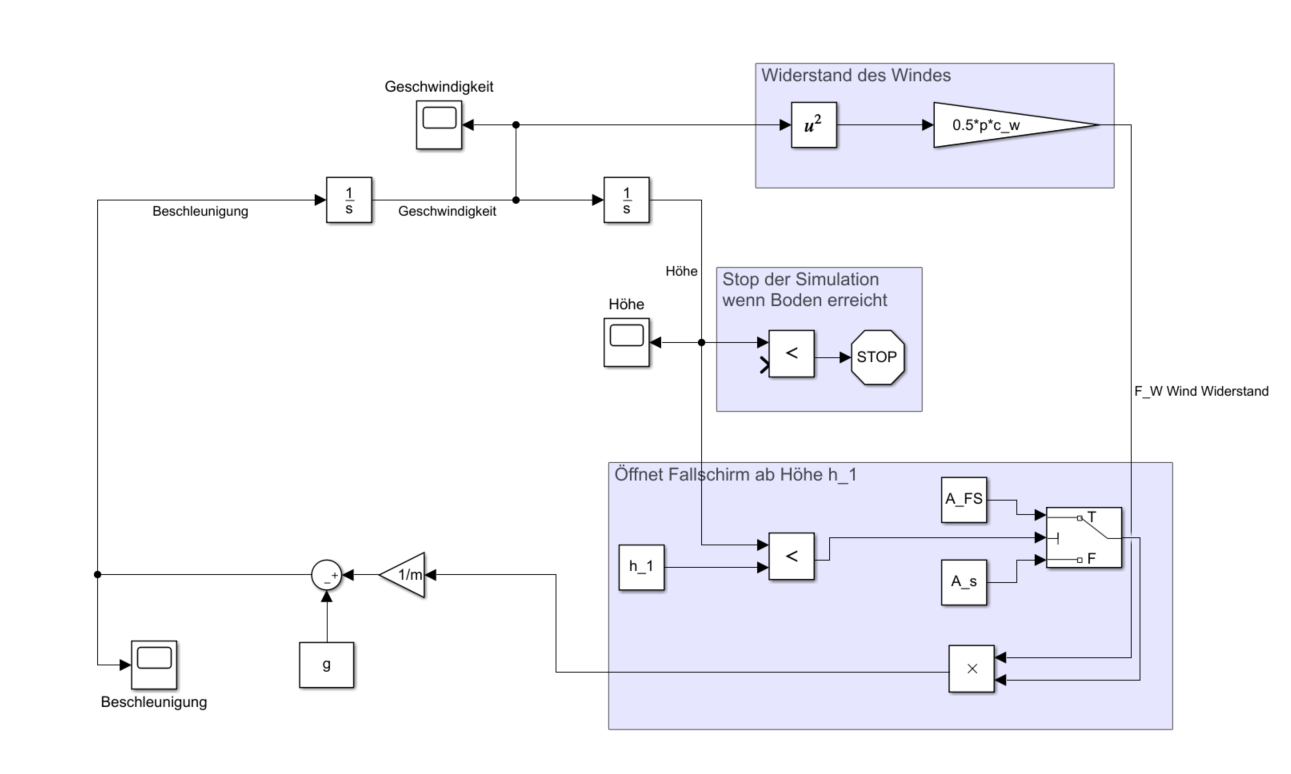
\includegraphics[width=\textwidth]{graphics/parachute_simulink.png}
    \centering
    \caption{Das Fallschirm Modell in Simulink}
    \label{abb:parachute_simulink}
\end{figure}

Das gleiche Modell, nun modelliert in Python, ergibt sich zu folgenden Quellcode,

\begin{lstlisting}[language=Python]
from control_theory.control_blocks import Integrator

if __name__ == '__main__':
    # Define constants
    h_0 = 3000
    h_1 = 1500
    A_s = 0.5
    A_FS = 25
    m = 85
    c_w = 1.3
    p = 1.2
    g = 9.81
    t, t_max, dt = 0, 500, 0.1

    # Define integrator objects
    a_integrator = Integrator()
    v_integrator = Integrator(initial_value=h_0)

    total_a = 0
    while t <= t_max:
        # Integrate acceleration and velocity
        total_a -= g
        v = a_integrator.integrate_signal(total_a)
        s = v_integrator.integrate_signal(v)

        # Stop if ground reached
        if s < 0:
            break

        # Wind resistance
        if s < h_1:
            F_w = v**2 * 0.5 * p * c_w * A_FS
        else:
            F_w = v**2 * 0.5 * p * c_w * A_s
        # Turn force into acceleration
        total_a = F_w / m

        t += dt

\end{lstlisting}

Zusehen ist, dass das Modell in Python angetrieben wird durch eine $while$-Schleife, welche terminiert, sobald das $t_{max}$ erreicht ist. Innerhalb der $while$-Schleife wird dafür die Laufvariable $t$ inkrementiert durch ein zuvor festgelegtes $dt$, welches in den zuvor erwähnten Integralen dem $\Delta t$ und somit der Integrationsschrittgröße entspricht. Konstanten wurden außerhalb der $while$-Schleife definiert zusammen mit einem $total\_a$, welches die gesamte Beschleunigung des Modells beschreibt. Die Integratoren werden nun innerhalb der $while$-Schleife verwendet, um die gesamte Beschleunigung in eine Geschwindigkeit und anschließend in die Höhe des Fallschirmspringers zu integrieren. Basierend auf diesen Methodenrückgaben können dann Veränderungen an den Signalen vorgenommen werden, um zum Beispiel das $F_W$ abhängig von der Höhe zu bestimmen. Ein direkter Vergleich der Ergebnisse unter Verwendung der gleichen Konstanten bei den beiden Modellvarianten in Python und Simulink zeigt dann auch gleich, dass die Integratoren und der Ansatz für die Modellierung in Python korrekt sind. Anzumerken ist jedoch, dass die Zeitachsen sich bei den beiden Plots ein wenig unterscheiden, dies ist jedoch darauf zurückzuführen, wie Simulink die Zeitschritte definiert und wie sie im Python Modell definiert sind. In diesem Fall ist es einfach nur eine unterschiedliche Skalierung.
\begin{figure}[H]
    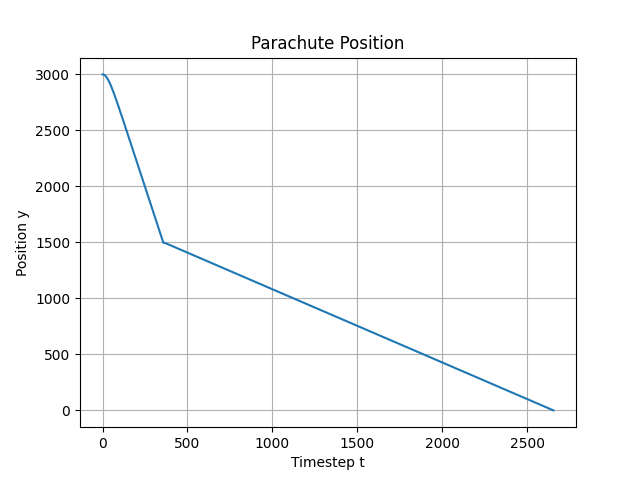
\includegraphics[width=\textwidth]{graphics/python_parachute_s_plot.png}
    \centering
    \caption{Plot der Höhe des Fallschirmspringers gegen die Zeit im Python Modell}
    \label{abb:python_parachute_s_plot}
\end{figure}

\begin{figure}[H]
    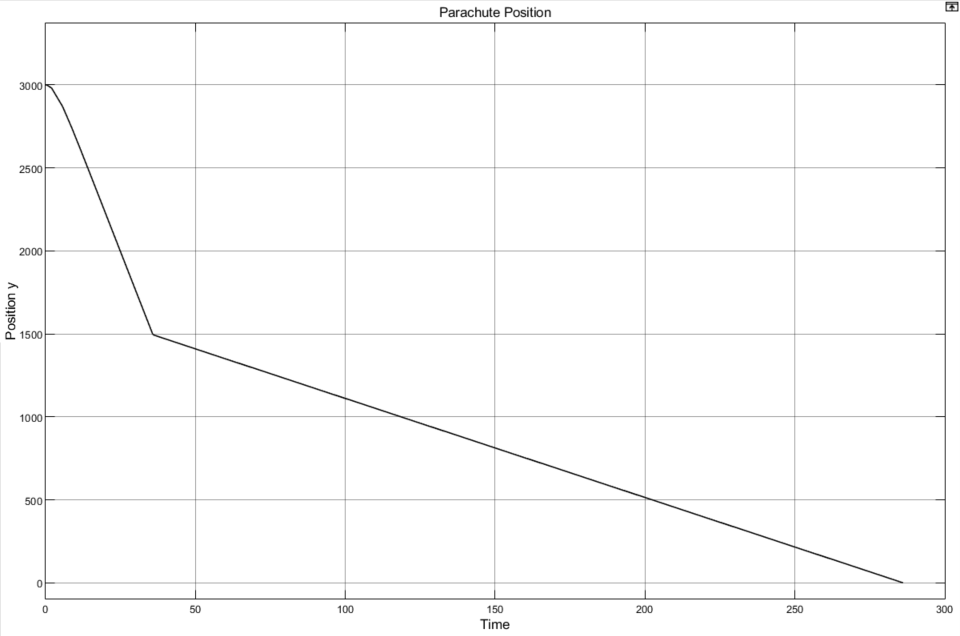
\includegraphics[width=\textwidth]{graphics/simulink_parachute_s_plot.png}
    \centering
    \caption{Plot der Höhe des Fallschirmspringers gegen die Zeit im Simulink Modell}
    \label{abb:simulink_parachute_s_plot}
\end{figure}

\subsection{Aufbau des Schiffmodells} \label{sec:aufbau_schiffsmodell}
Das nun in Simulink gebildete Modell soll zusammen mit den zuvor erwähnten Methoden in Python implementiert werden. Als Grundlage wird hierfür ein Environment aus der Gym Bibliothek von OpenAI verwendet. Das gesamte Modell wird innerhalb der \textit{BoatEnv} Klasse definiert, welche von der Grundklasse für Environments aus Gym erbt. Gym schreibt einige Klassenattribute und Klassenmethoden vor, welche auf jeden Fall neu definiert werden müssen, damit das Environment von alleine funktionieren kann.

Das erste Klassenattribut ist der Actionspace, welcher dem Agenten seine möglichen Actions gibt, welche er durchführen kann. Da in dieser Arbeit der Agent das Schiff lediglich mit dem Rudern kontrollieren soll, wurde aus diesem Grund auch nur ein 1-Dimensionaler Actionsspace definiert, welcher eine Reichweite von $-1$ bis $1$ besitzt. An dieser Stelle ist es wichtig, dass außerdem der Actionsspace in einem von Gym vordefinierten \textit{Box}-Space definiert wird, da dies dafür sorgt, dass der Actionsspace auch tatsächlich kontinuierlich ist. Im weiteren Verlauf wurde festgestellt, dass die Reichweite des Actionsspaces zu extrem für die Regelung des Schiffes ist. Der Agent ist in Prinzip in der Lage, das Ruder von einem auf den andern Moment um $\SI{1}{\radian}$ zu bewegen, was bereits ziemlich realitätsfern ist. Da eine direkte Herunterskalierung der Reichweite des Actionsspaces selbst jedoch dazu führt, dass der SAC nicht mehr richtig funktioniert, beziehungsweise instabil wird. Stattdessen wird als Lösungsweg, die vom SAC gewählte Action durch 10 geteilt, um eine Herunterskalierung zu erlangen.

Das zweite Klassenattribut, welches nun überschrieben beziehungsweise neudefiniert wurde, ist der Observationsspace. Für diese Arbeit wurde ein ziemlich großer Observationsspace gewählt, um dem Agenten somit möglichst viele Informationen geben zu können. Auch in diesem Fall wurde analog zum Actionsspace das vordefinierte \textit{Box}-Space verwendet, um Kontinuität zu besitzen. Es wurde ein Observationspace verwendet, welcher die folgenden Informationen über das Environment trägt,
\begin{enumerate}
    \item[-] Schiffsposition und Ausrichtung $(s_x, s_y, s_r)$
    \item[-] Schiffgeschwindigkeit und Winkelgeschwindigkeit $(v_x, v_y, v_r)$
    \item[-] Schiffbeschleunigung und Winkelbeschleunigung $(a_x, a_y, a_r)$
    \item[-] Ausrichtung des Ruders und restlicher Treibstoff $(\alpha, f_{uel})$
\end{enumerate}
Die Größen der einzelnen Informationen wurden auf einen Bereich von $0$ bis $1$ normiert, da neuronale Netzwerke und somit der Agent dadurch deutlich effizienter funktionieren können. \cite[]{normalization_importance}

Ein Gym Environment besitzt nun eine Reihe an Klassenmethoden, welche zusätzlich neben dem Actionsspace und dem Observationsspace implementiert werden müssen, damit ein Environment auch vollständig funktionieren kann. Die wichtigsten Klassenmethoden sind in diesem Fall die \textit{step} und \textit{reset} Methoden. Es gibt noch weitere, wie \textit{render}, diese wurden allerdings nicht verwendet beziehungsweise selbst auf anderem Wege implementiert.

Die \textit{step} Methode ist die Klassenmethode, welche dafür sorgt, dass innerhalb einer Episode auch ein Schritt ausgeführt werden kann. Als Argument besitzt die Methode die Action, welche vom Agenten gewählt wurde. Das heißt, wenn der Agent eine Winkeländerung des Ruders von $\SI{0.2}{\radian}$ vornehmen möchte, sorgt diese Methode jetzt dafür, dass auch das Modell demnach angepasst wird und ein Simulationsschritt ausgeführt wird. Die Simulation des Schiffs, welche unter anderem durch die \textit{step} Methode angetrieben wird, wurde implementiert innerhalb einer eigenen Klasse, auf welche zusammen mit dem Wind später eingegangen werden soll. Während eines Schrittes innerhalb einer Episode wird auch der Reward berechnet, welcher der Agent nun erhält, für die Action und dem State in welchen er das Environment gebracht hat. Für die Berechnung des Rewards, wurde eine Reward Function Klasse konstruiert, welche abhängig davon wo das Schiff sich momentan befindet einen Reward bestimmt. Bei der Entwicklung und Visualisierung der mathematischen Funktionen, welche den Reward berechnen, wurde der Online Grafikrechner Desmos \cite[]{desmos} verwendet. Der in dieser Arbeit verwendete Reward wird abhängig von der aktuellen Position in der y-Achse berechnet durch,
\begin{align}
    r & = -f_y(s_y)                                                          \\
      & = - \frac{\frac{|s_y|}{g_b}}{1 + e^{\frac{-a}{b}(|s_y| - 0.2 g_w)}}.
\end{align}
Es wurde zuvor damit experimentiert außerdem die Position in der x-Achse zu verwenden, jedoch sorgte dieses für eine Rewardverteilung welche nahe der Ziellinie zu viele positive Punkte am Rand des Spielfeldes gibt. Ein Resultat dadurch war, dass der Agent nicht stark genug am Rand bestraft wurde und ihn somit vermehrt ansteuerte und es zu frühzeitigen Episoden Beendungen kam. Stattdessen wird nun nur noch die y-Position verwendet, welche zu einer Rewardverteilung wie in Abbildung \ref{abb:reward_field} führt.

\begin{figure}[H]
    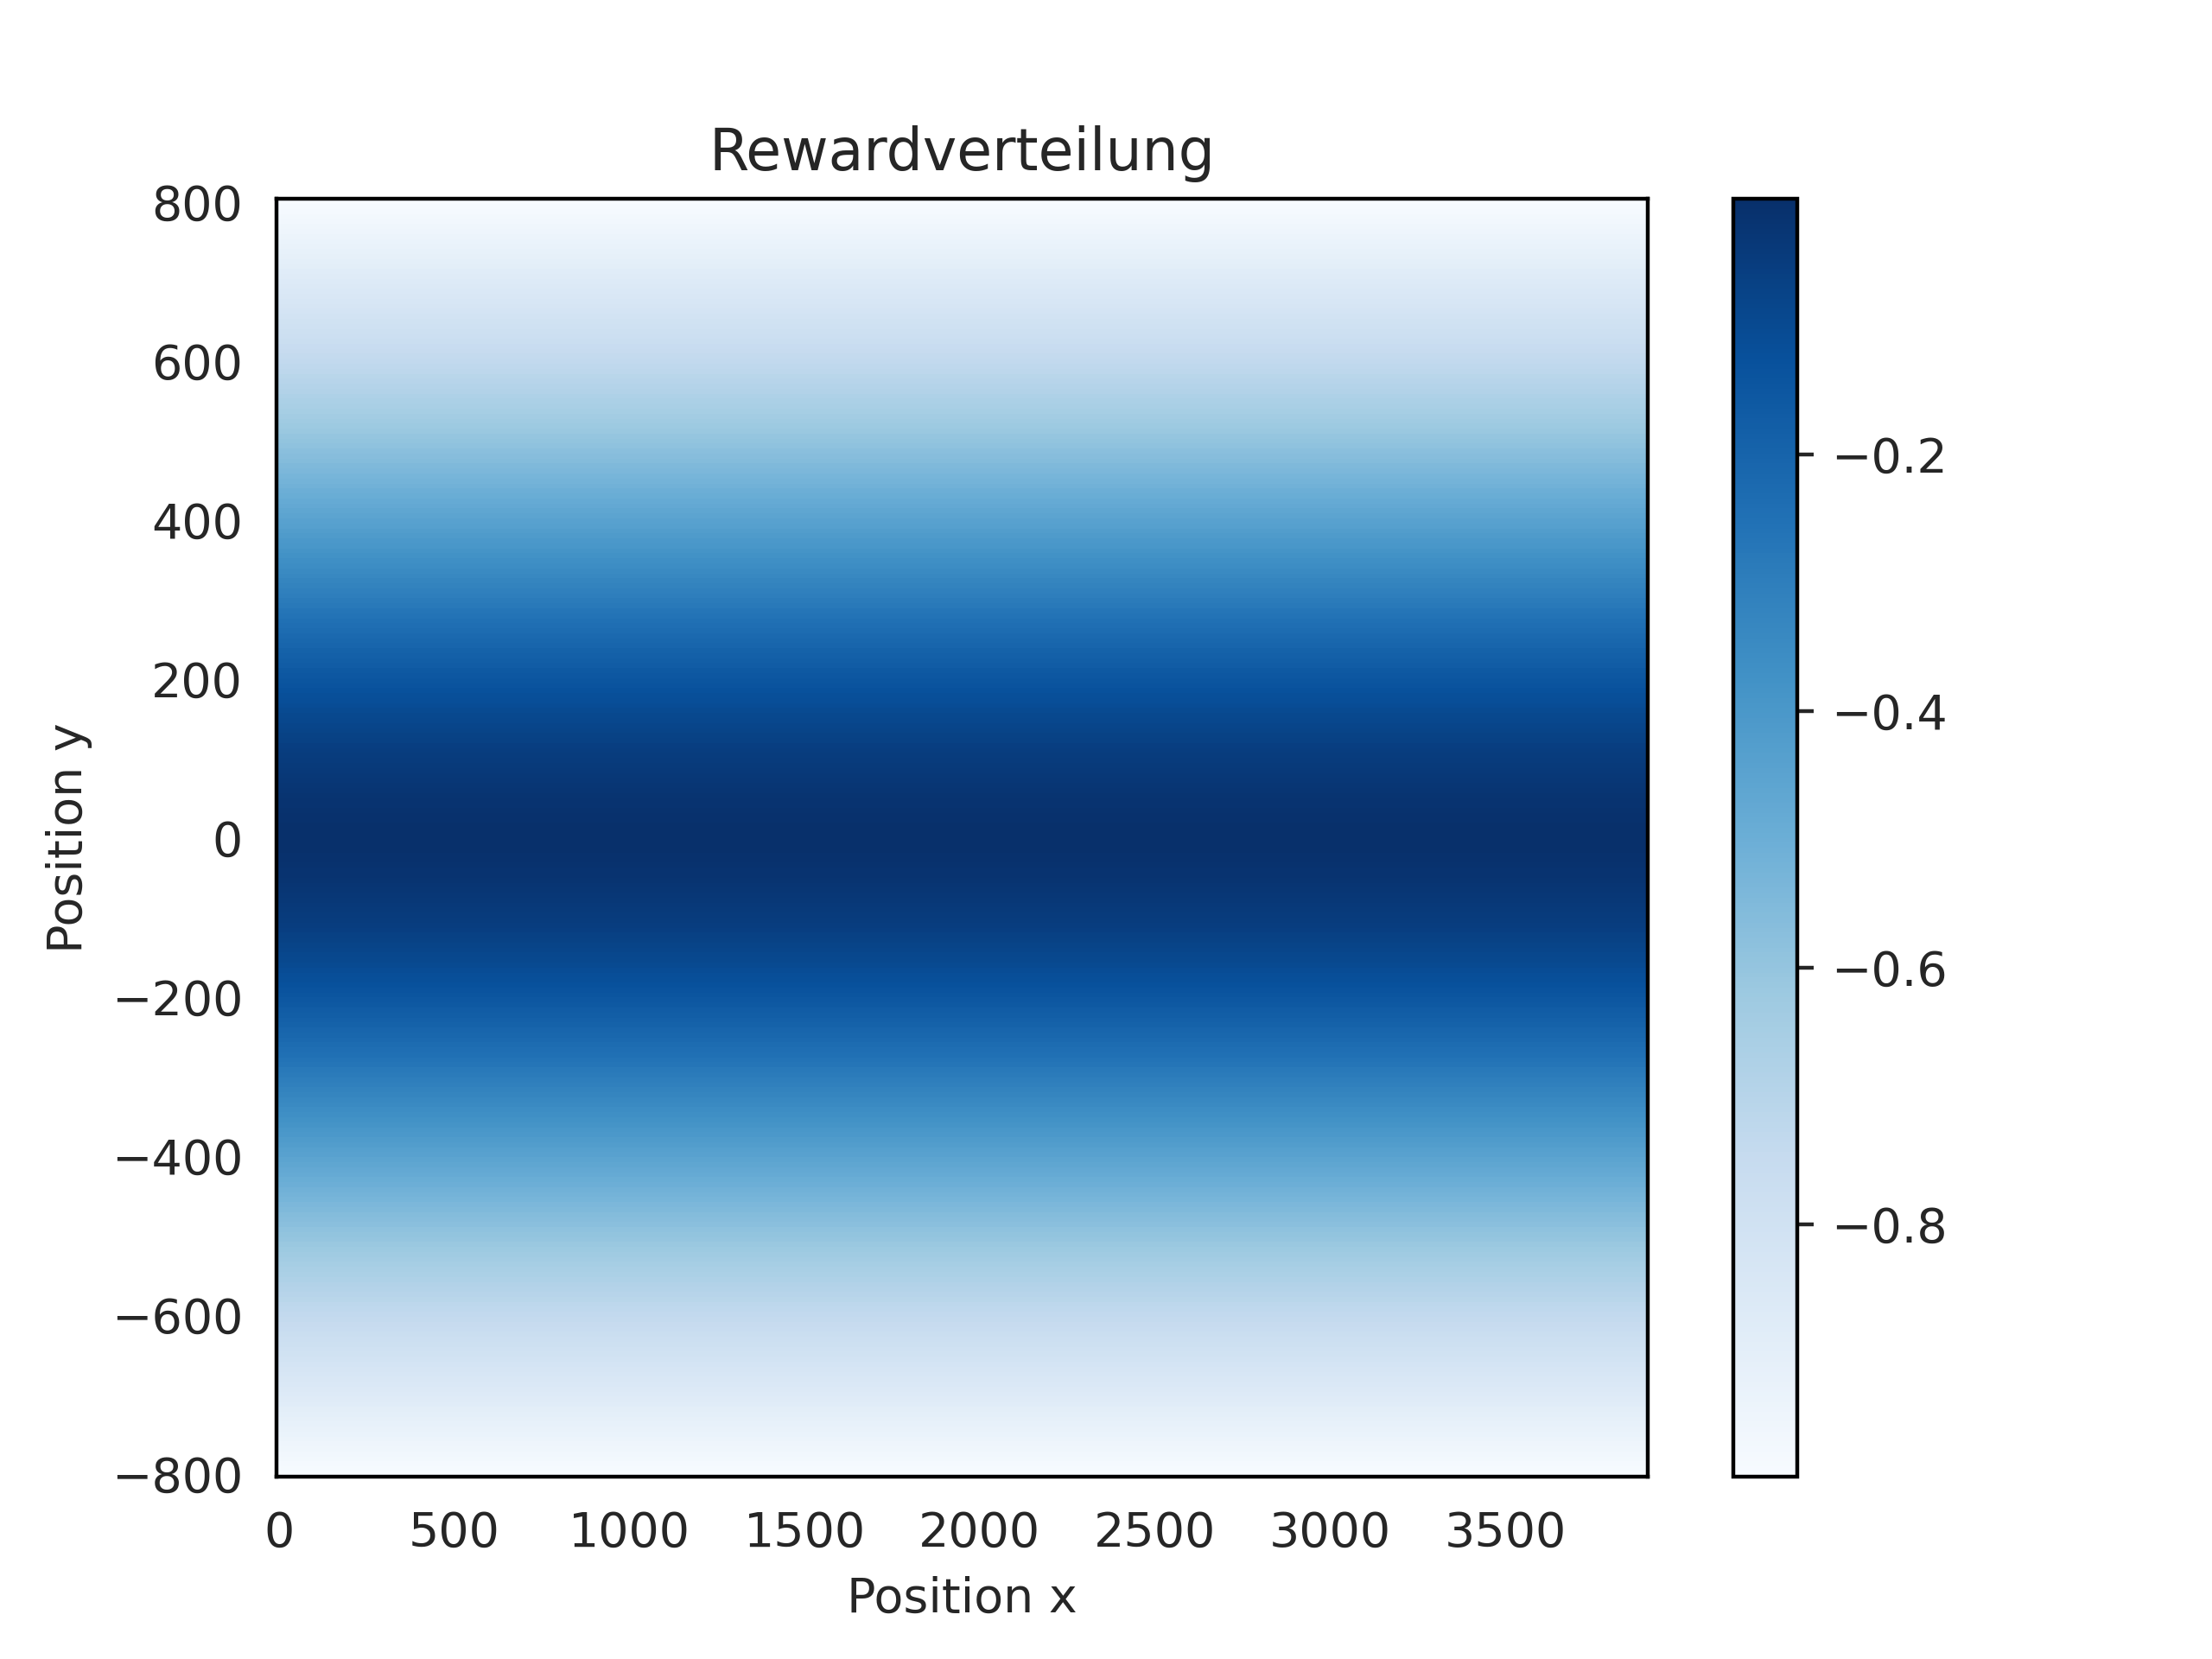
\includegraphics[width=\textwidth]{graphics/reward_field.png}
    \centering
    \caption{Visualisierung der Rewardverteilung über das gesamte Spielfeld des Schiffmodells.}
    \label{abb:reward_field}
\end{figure}

Erkennbar in Abbildung \ref{abb:reward_field} ist nun, dass der Reward für den Agenten dauerhaft so gewählt ist, dass er zwangsweise in der Mitte des Spielfeldes bleiben muss, um nicht bestraft zu werden. Bewegt er sich von der Mitte weg, so wird er immer stärker bestraft.

Es wurde zuvor bereits angedeutet, dass der Agent auch für seine ausgeführte Action einen Reward bekommt. Das Modell wurde so gebildet, dass sich das Ruder nicht außerhalb eines Winkels von $-\frac{\pi}{3} \leq \alpha \leq \frac{\pi}{3}$ befinden darf. Es wurde somit eine Bestrafung eingeführt für den Agenten, wenn er eine Action wählt, welche das Ruder in einen Winkel von $-\frac{\pi}{4} \leq \alpha \leq \frac{\pi}{4}$ setzen würde. Die Bestrafung wird hierbei linear größer, je weiter sich der Agent dem wirklichen Winkel nähert, welcher das Ruder zerstören würde. Erreicht der Agent die $-\frac{\pi}{3} \leq \alpha \leq \frac{\pi}{3}$ Grenze, so wird die Episode frühzeitig beendet. Des Weiteren wird der Agent dafür bestraft, dass er das Schiff so umlenkt, dass es von rechts nach links fahren würde. Eine positive Belohnung wird verteilt, wenn er erfolgreich die Ziellinie erreicht.

Die folgende Liste, soll noch einmal darstellen, welche Kriterien existieren, die zu einer frühzeitigen (-) oder erfolgreichen (+) Beendigung einer Episode führen,
\begin{enumerate}
    \item[+] Das Schiff fährt in die Ziellinie
    \item[-] Das Schiff fährt gegen den Rand des Spielfeldes
    \item[-] Das Schiff besitzt keinen Treibstoff mehr
    \item[-] Die maximale Simulationszeit wurde überschritten
    \item[-] Das Ruder wurde zerstört
\end{enumerate}

Die letzte Klassenmethode aus dem Gym Environment, welche noch neudefiniert werden musste, ist die \textit{reset} Methode. Die Aufgabe dieser Methode ist es, das komplette Environment wieder in seinen Ursprungsstate zurückzusetzen. Hier werden also Aufgaben übernommen, wie die Generierung von neuen Windparametern, das Zurücksetzen des Schiffes auf den Ursprung und das Zurücksetzen der gesammelten Rewards dieser Episode.

Die gesamte Simulation beziehungsweise das Modell des Schiffes wurde in eine gebundene Klasse implementiert. Das Ziel hierbei ist, die Übersicht klar zuhalten im Sinne der Softwareentwicklung, und außerdem eine Kapselung und damit Modularität zu besitzen. Innerhalb dieser Klasse finden sich nun unter anderem all die Integratoren, wie sie in Kapitel \ref{sec:integrator_test} beschrieben wurden. Analog zum Beispiel mit dem Fallschirmspringer, welcher vorgestellt wurde, um die in Python implementierten Integratoren zu testen, wurden auch hier erneut Klassenattribute verwendet, um die verschiedenen Laufvariablen für die Simulation zu definieren. Die drei Bewegungsgleichungen wurden jeweils in eine eigene Klassenmethode umgesetzt, welche beim Aufrufen aus einer \textit{run} Methode die Klassenattribute dementsprechend anpassen und einen Zeitschritt in der Simulation ausführen. Auch die Normalisierung der Werte, welche für den Observationsspace benötigt werden, wird hier durchgeführt. Die Maxima und Minima der jeweiligen Werte wurden experimentell in Simulink bestimmt, und innerhalb des Python-Modells als feste Werte verwendet. Im Beispiel des Fallschirmspringers wurde eine $while$-Schleife verwendet, um die gesamte Simulation anzutreiben. Diese existiert in diesem Fall nicht, da die Simulation von außerhalb mit der \textit{step} Methode des Gym Environments angetrieben wird und somit nur für die Länge einer Episode existiert bis sie zurückgesetzt wird. Es wurde dennoch eine maximale Laufzeit $t_{max}$ zusammen mit einer aktuellen Zeit $t$ implementiert. Diese dienen jedoch nur dazu, um sicherzustellen, dass das Modell auch wirklich beendet wird, falls von außerhalb Komplikationen unabhängig von der Simulation auftreten. Die Zeit $t$ wird außerdem verwendet, um Zugriff auf die Größen des Windes zu haben, welche per Index in diversen Listen gespeichert sind.

Der Wind wurde wie auch die Simulation des Schiffes ausgelagert in eine eigene Klasse, für eine bessere Übersicht und mehr Kontrolle über die gewollten Eigenschaften des Windes. Im Grunde ist das Hauptziel der Wind-Klasse, die Möglichkeit zu bieten, alle sechs gewollten Wind Konfigurationen zu erstellen. Es wurde somit eine Klassenmethode erstellt, welche abhängig von einem Parameter, welcher in einer Konfigurationsdatei gesetzt werden kann, einen jeweiligen Wind erstellt. Einige Konfigurationen verlangen nach Kurvenverläufen, welche eine rein zufällig erstellt werden müssen. Hierfür wurde eine Hilfsmethode implementiert, welche $n$ Punkte mit gleichem Abstand in einer Reihe generiert. Die einzelnen Punkte, welche gesetzt wurden und einen zufälligen Wert zwischen 0 und 1 besitzen, werden dann abschließend per kubischen Interpolation miteinander verbunden.

\section{Training und Hyperparameteroptimierung}
Innerhalb dieser Arbeit wurden insgesamt sechs Experimente untersucht, auf die Details der einzelnen Experimente und was genau mit ihnen überprüft wird, soll im nächsten Kapitel eingegangen werden. Dennoch soll jetzt schon einmal darauf eingegangen werden, wie nun das tatsächliche Trainieren der Agenten stattgefunden hat und wie zum Beispiel die Hyperparameter des SAC Agenten gewählt wurden.

Algorithmen aus dem maschinellen Lernen besitzen in den meisten Fällen immer eine bestimmte Menge an Eigenschaften, welche sehr großen Einfluss auf die Performanz haben. So können neuronale Netzwerke zum Beispiel mit verschiedenen Anzahlen an Schichten erstellt werden, hinzu kommt, dass dann auch noch die Breiten der einzelnen Schichten gewählt werden können, was für eine Aktivierungsfunktion verwendet wird und viele andere Einstellungen. Diese Eigenschaften oder Einstellungen, welche hier gewählt werden können, werden in der Literatur oft als sogenannte Hyperparameter bezeichnet. Wird erneut das neuronale Netzwerk Beispiel verwendet und es wird außerdem angenommen, dass nun kein Vorwissen über diese Hyperparameter und deren Einfluss besteht, so kommt die Frage auf, wie diese nun an besten gewählt werden sollen. Es besteht immerhin ein Wunsch danach, das optimale Set an Hyperparametern zu verwenden, da ihr Einfluss auf die Ergebnisse so groß ist. Es hilft an dieser Stelle oft, bereits eine gewisse Menge an Vorerfahrung mitzubringen, umso die Möglichkeit zu besitzen aus eigenem Wissen abschätzen zu können, was für eine Breite an besten passt, oder wie viele Schichten notwendig sind. Dennoch wird es wahrscheinlich sein, dass die Gesetzen Hyperparameter dann immer noch nicht das Optimum bilden.

Abhilfe für dieses Problem soll die Hyperparameteroptimierung bieten. Das Ziel einer solchen Optimierung ist es, per automatischen Verfahren ein optimales oder fast optimales Set an Hyperparametern bestimmen. Es gibt eine ganze Anzahl an verschiedenen Verfahren, wie eine solche Optimierung nun funktionieren kann. Letztendlich basieren sie allerdings alle darauf, dass viele Modelle oder Agenten trainieren werden müssen, mit verschiedenen Parametern und anschließend eine Auswertung stattfindet, um das bisher beste Ergebnis zu finden. Ansätze können unter anderem darauf basieren, dass vorherige Ergebnisse und deren Hyperparameter Sets gespeichert werden und die neuen Sets auf Basis von Wahrscheinlichkeiten neu generiert werden. Existiert dabei ein Trend, dass gewisse Hyperparameter gute Ergebnisse liefern, so wählt ein Optimierer automatisch ein neues Set mit ähnlichen Hyperparametern.

Der Ansatz, welcher in dieser Arbeit verwendet wurde, basiert jedoch auf eine komplett zufällige Suche. Die folgende Tabelle gibt eine Übersicht, welche Hyperparameter angepasst werden,
\begin{table}[H]
    \begin{tabular}{l|l}
        Learning Rate:                & $0.001 \leq \alpha \leq 0.01$  \\ \hline
        Learning Rate:                & $0.0008 \leq \beta \leq 0.008$ \\ \hline
        Target Smoothing Coefficient: & $0.001 \leq \tau \leq 0.01$    \\ \hline
        Discount Factor:              & $0.95 \leq \gamma \leq 0.99$
    \end{tabular}
    \caption{Eine Übersicht der verschiedenen Hyperparameter, welche in dieser Arbeit beim Trainieren des SAC dynamisch angepasst wurden.}
    \label{tab:hps}
\end{table}
Die Learning Rates $\alpha$ und $\gamma$ dienen dazu, die Optimierer in den neuronalen Netzwerken anzupassen. Die Learning Rate $\alpha$ passt dabei das Policy Netzwerk an, während $\beta$ die Optimierer der restlichen Netzwerke anpassen. Der Target Smoothing Coefficient dient dazu bei dem überschreiben der Value und Target-Value Netzwerke eine gewisse Menge an Streuung einzubringen, welche dazu führt, es weniger Abweichungen innerhalb der Netzwerke gibt und somit ein Overfitting unwahrscheinlicher wird. \cite[]{https://doi.org/10.48550/arxiv.1802.09477} Der Discount Factor ist jener Wert, welcher bereits in der Theorie in den Gleichungen \ref{eq:finite_horizon_undiscounted} und \ref{eq:infinite_horizon_discounted} erwähnt wurde.

Das Trainieren der Agenten wurde nun so durchgeführt, dass zuerst ein Experiment gewählt wurde und dessen Einstellungen eingespielt wurden. Anschließend wird das Training gestartet für eine bestimmte Anzahl an Durchläufen. Ein Durchlauf besitzt eine Länge von insgesamt 250 Episoden und es wird ein Hyperparameter Set zufällig aus den Reichweiten gewählt. Das Training des Agenten wird durchgeführt, bis es vollendet und es wird neu gestartet. Im Schnitt dauerte das Training eines einzelnen Durchlaufes mit 250 Episoden etwa 5 Stunden, wobei hier immer 5 Agenten gleichzeitig auf derselben Hardware trainiert wurden.

\chapter{Experimente und Ergebnisse TODO} \label{sec:ergebnisse}
Im folgenden Kapitel werden die Experimente vorgestellt, welche mit der kompletten Implementierung des Agenten und seinem Environments durchgeführt wurden. Nach der Vorstellung der Experimente folgt dann abschließend die Präsentation der Ergebnisse mit der dazugehörigen Auswertung.

\section{Experimente}
Für diese Arbeit wurde die Untersuchung des dynamischen Modells und seiner Regelung durch einen SAC Agenten in insgesamt sechs Experimente aufgeteilt. Die Experimente befassen sich dabei in jeder Instanz darum, inwiefern der Agent in der Lage ist, das Schiff von der Startposition in die Ziellinie zuführen. Unterschieden wird zwischen den Experimenten dadurch, inwiefern die Störgröße von außen kontrolliert wird, welche den Agenten aus seiner Fahrbahn bringen soll. Das erste Experiment fängt ziemlich leicht an, schrittweise werden sie jedoch schwieriger. Somit soll das Limit des Agenten getestet werden, um herauszufinden, wo gegebenenfalls mehr Untersuchungen vonnöten sind, um den Agenten oder die Methodik selbst zu verbessern.

Grundsätzlich gibt es dennoch gleichbleibende Einstellung bei den unterschiedlichen Experimenten. In jedem Experiment wurde dieselbe Rewardverteilung verwendet, wie sie bereits in Abbildung \ref{abb:reward_field} vorgestellt wurde. Außerdem sind die Eigenschaften des Spielbrettes selbst gleichbleibend. So wurde die Ziellinie immer bei 5900 auf der x-Achse gesetzt. Die Spielbrettbreite ist auch stetig so gewählt, dass die insgesamt 800 Einheiten groß ist. Die Koeffizienten und Größen, welche für die Modellierung des Schiffs verwendet wurden, verändern sich mit den Experimenten nicht.

Die Abbildungen, welche hier in den einzelnen Experimenten verwendet werden, um unter anderen die Windeigenschaften zu visualisieren, wurden ohne Einfluss eines SAC Agenten generiert. Hier wurde nur eine konstante Propeller-Drehgeschwindigkeit gesetzt, um den Einfluss des Windes auf das Schiff zu erkennbar zu machen.

\subsection*{Experiment 1}
Das erste Experiment ist sehr einfach gehalten. Das Ziel ist es hier, die Ziellinie zu erreichen, ohne dass überhaupt eine Störgröße von Außen auf das Schiff wirkt. Der Wind ist hier komplett deaktiviert und das Schiff startet in der regulären Startposition, welches links auf dem Spielbrett liegt. Das Ziel dieses Experiments ist es vor allem zu überprüfen, ob der Agent überhaupt in der Lage ist, das Schiff in seiner Grundform ohne von außen wirkenden Störungen zu regeln. Es dient außerdem als eine Testumgebung, in welcher die Grundeinstellungen des Schiffs überprüft werden können, bevor später zu schwierigeren Szenarien übergegangen wird. So wurden hier unter anderem die Rewardverteilungen getestet, oder welche Kriterien für frühzeitige Beendungen sich wirklich lohnen.
\subsection*{Experiment 2}
Das zweite Experiment ist in Prinzip dem ersten Experiment ziemlich gleich. Auch hier weht aus keiner Richtung ein Wind als Störgröße. Der Unterschied liegt nur darin, dass hier die Startposition des Schiffes ein wenig variiert wird. Die Startposition wird hier auch links vom Spielfeld gewählt, jedoch wird zufällig eine Position der y-Achse gewählt. Es existiert hierbei eine oberere und unterere Grenze, in welcher das Schiff platziert werden kann, damit es nicht zu nah am äußeren Rand liegt und gewissen Spielraum hat noch irgendwie in die Mitte zu kommen. Ziel dieses Experiments soll es sein zu untersuchen, wie schnell der Agent in der Lage ist, das Schiff wieder in die Mitte des Spielbrettes zu kommen, um anschließend erfolgreich die Ziellinie zu erreichen. Ein Beispiel wie das Schiff in einem Experiment dieser Schwierigkeitsstufe startet, ist zu erkennen in der folgenden Abbildung,
\begin{figure}[H]
    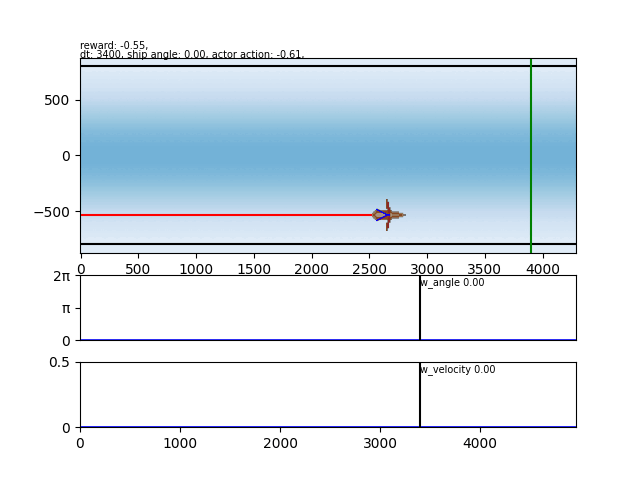
\includegraphics[width=\textwidth]{graphics/settings/s2.png}
    \centering
    \caption{Ein Beispiel Ausschnitt von einem Experiment mit Schwierigkeitsstufe 2, deutlich zu erkennen ist, dass hier kein Wind weht und das Schiff in einer weit verschobenen Position nach unten beginnt.}
    \label{abb:setting2}
\end{figure}
\subsection*{Experiment 3}
Innerhalb des dritten Experiments wird das erste Mal untersucht, inwiefern der Agent auf den Wind reagiert. Für dieses Experiment soll der Wind jedoch nur aus einer Richtung wehen und stetig mit gleicher Geschwindigkeit. Die Windrichtung wird hier so gewählt, dass sie von unten nach oben im Spielbrett weht. Es wird eine konstante Geschwindigkeit von $\SI{0.5}{\m\per\s}$. Diese Größe wurde so gewählt, da sie durch Versuche gezeigt hat, dass sie einen vernünftigen Einfluss auf das Schiff hat, aber nicht so groß ist, dass der Agent überhaupt keine Chance hat dagegen wirken zu können. Die Startposition wird mit diesem Experiment nicht mehr variiert wie es im vorherigen Experiment der Fall war. Die folgende Abbildung zeigt wie der Wind das Schiff konstant von der Bahn schiebt,
\begin{figure}[H]
    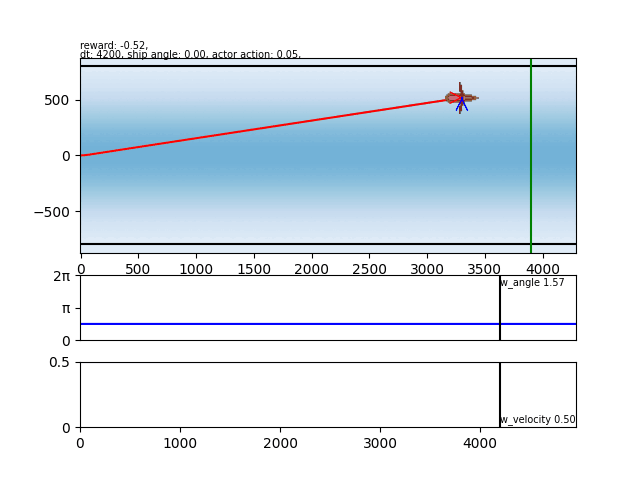
\includegraphics[width=\textwidth]{graphics/settings/s3.png}
    \centering
    \caption{Das dritte Experiment, welches mit konstanter Windgeschwindigkeit das Schiff deutlich zu erkennen aus der Bahn nach außen drückt.}
    \label{abb:setting3}
\end{figure}
\subsection*{Experiment 4}
Mit dem vierten Experiment wird das dritte Experiment noch einmal schwieriger, indem nun außerdem die Windgeschwindigkeit fluktuiert und nicht mehr konstant bei $\SI{0.5}{\m\per\s}$ gehalten wird. Die Windrichtung wird erneut so gewählt, dass er von unten nach oben weht, hingegen wird die Windgeschwindigkeit jetzt zufällig in einem Bereich von $\SI{0}{\m\per\s}$ bis $\SI{0.5}{\m\per\s}$ gesetzt. Ein Beispiel zum Verlauf des Windes ist zu erkennen in der folgenden Abbildung \ref{abb:setting4},
\begin{figure}[H]
    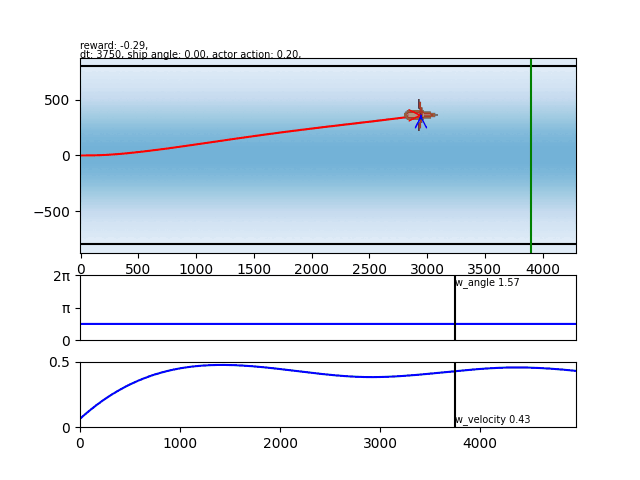
\includegraphics[width=\textwidth]{graphics/settings/s4.png}
    \centering
    \caption{Ein Ausschnitt, wie das Initiale State aus einem Experiment mit Schwierigkeitsstufe 4 aussieht. Hier zu erkennen, wie der Wind mit variierender Geschwindigkeit auf das Schiff wirken wird innerhalb der Episode.}
    \label{abb:setting4}
\end{figure}
In diesem Beispiel ist unter anderem zu erkennen, dass der Wind zum Beginn der Episode recht milde weht, hingegen wird er gegen Ende sehr vergleichsweise stark sein.

\subsection*{Experiment 5}
Das fünfte Experiment hat das Ziel, das erste Mal zu untersuchen, wie nun der Agent auf verschiedene Windrichtungen wirkt. Die Richtung ist jedoch noch immer in einem limitieren Bereich definiert. Innerhalb dieses Experiments soll er nämlich nur von entweder oben nach unten oder unten nach oben wehen. Er verfügt somit nicht die Möglichkeit das Schiff irgendwie in der longitudinalen Richtung zu beschleunigen, kann es jedoch trotzdem jetzt in zwei Richtungen von der Bahn lenken. Für dieses Experiment wird der Wind jedoch so gewählt, dass er erneut eine strickte Geschwindigkeit von $\SI{0.5}{\m\per\s}$ besitzt. Abbildung \ref{abb:setting4} soll zeigen, wie der Wind in diesem Fall aussehen würde, wenn er zufällig generiert wird.
\begin{figure}[H]
    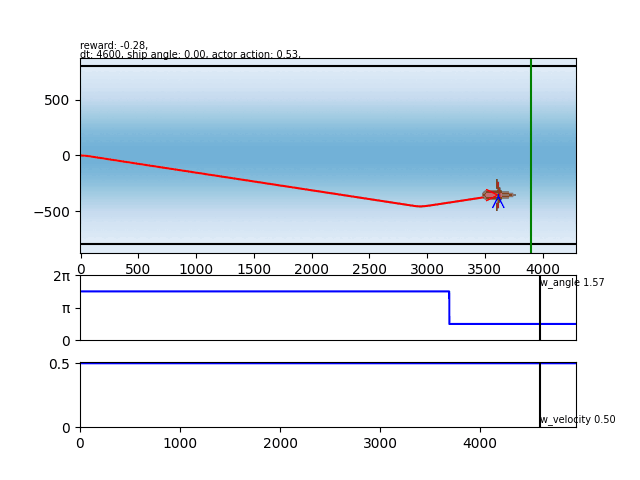
\includegraphics[width=\textwidth]{graphics/settings/s5.png}
    \centering
    \caption{Ein Experiment mit Schwierigkeitsstufe 5, hier unter anderem zu erkennen, wie der Wind die Form einer Rechteckkurve annimmt, da er lediglich aus zwei Richtungen wehen kann.}
    \label{abb:setting5}
\end{figure}

\subsection*{Experiment 6}
Das letzte und schwierigste Experiment soll aus den vorherigen Experimenten allerlei Elemente zusammenfassen. Die einzige Eigenschaft, welche hier nicht übernommen wurde, ist die der verschobenen Anfangspositionen. Da hier ein Wind aus allen Richtungen wehen kann, kam es bei ersten Versuchen oft zu der Situation, dass das Schiff innerhalb von nur wenigen Schritten schon aus dem Spielfeld geschoben wurde. Dem SAC Agenten war es somit gar nicht möglich, überhaupt eine Regelung vorzunehmen. Die anderen Eigenschaften werden jedoch übernommen, es ist somit nun möglich, dass der Wind mit variierender Geschwindigkeit aus allen Richtungen wehen kann. Das Schiff kann also von der Bahn gelenkt werden und außerdem eine Beschleunigung in longitudinaler Richtung erfahren. Ein Ausschnitt, der nun zeigt, wie dies aussieht, findet sich in Abbildung \ref{abb:setting6},
\begin{figure}[H]
    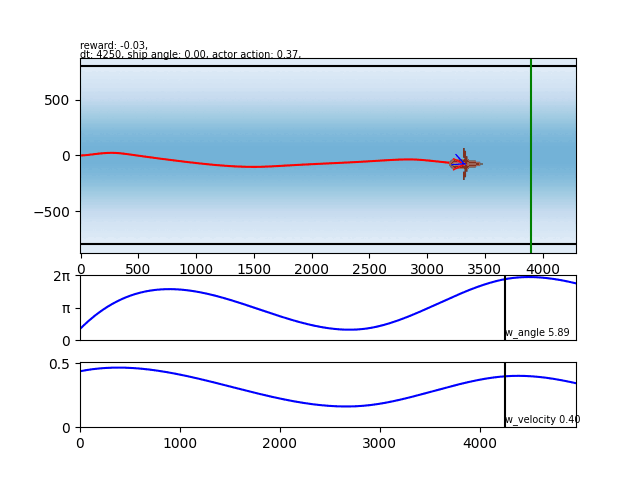
\includegraphics[width=\textwidth]{graphics/settings/s6.png}
    \centering
    \caption{Das Experiment der Schwierigkeitsstufe 6, hier zu erkennen, wie der Wind nun aus allen Richtungen wehen kann und seine Geschwindigkeit variabel ist.}
    \label{abb:setting6}
\end{figure}

\section{Ergebnisse und Auswertung}

\chapter{Diskussion TODO} \label{sec:diskussion}

\chapter{Zusammenfassung und Ausblick TODO} \label{sec:zsmfassung_ausblick}


\printbibliography

\end{document}